\documentclass{article}
\usepackage[utf8]{inputenc}
\usepackage[fontsize=13pt]{scrextend}
\usepackage{geometry}
\usepackage{multicol}
\usepackage{xeCJK} 
\usepackage{lmodern} % For scalable Computer Modern fonts
\usepackage[T1]{fontenc} % Ensures proper font encoding
\usepackage{color}
\usepackage{helvet}  % For changing fonts

\usepackage{soul}  % For highlighting

\geometry{
  a4paper,
  left=25mm,
  right=25mm,
  top=25mm,
  bottom=25mm,
  heightrounded,
}
\usepackage[T1]{fontenc}
\usepackage{amsmath}
\usepackage{amsfonts}
\usepackage{amssymb}
\usepackage{graphicx}
\usepackage{tabularx}
\usepackage{lastpage}
\usepackage{xcolor}
\usepackage{tikz}
\usepackage{pgfplots}
\usepackage{hyperref}
\usepackage{listings}
\usepackage{booktabs}
\usepackage{tabularray}
\usepackage{multirow}
\usepackage{float}
\usepackage{lastpage}
\usepackage{tcolorbox}
\usepackage{titlesec}

\usepackage{etoolbox}

\makeatletter
\patchcmd{\@zfancyhead}{\fancy@reset}{\f@nch@reset}{}{}
\patchcmd{\@set@em@up}{\f@ncyolh}{\f@nch@olh}{}{}
\patchcmd{\@set@em@up}{\f@ncyolh}{\f@nch@olh}{}{}
\patchcmd{\@set@em@up}{\f@ncyorh}{\f@nch@orh}{}{}
\makeatother



\usepackage{lastpage} % Required to determine the last page number for the footer

\usepackage{graphicx} % Required to insert images

\setlength\parindent{0pt} % Removes all indentation from paragraphs

\usepackage[most]{tcolorbox} % Required for boxes that split across pages

\usepackage{booktabs} % Required for better horizontal rules in tables

\usepackage{listings} % Required for insertion of code

\usepackage{etoolbox} % Required for if statements

%----------------------------------------------------------------------------------------
%	MARGINS
%----------------------------------------------------------------------------------------

\usepackage{geometry} % Required for adjusting page dimensions and margins

\geometry{
	paper=a4paper, % Change to letterpaper for US letter
	top=3cm, % Top margin
	bottom=3cm, % Bottom margin
	left=2.5cm, % Left margin
	right=2.5cm, % Right margin
	headheight=14pt, % Header height
	footskip=1.4cm, % Space from the bottom margin to the baseline of the footer
	headsep=1.2cm, % Space from the top margin to the baseline of the header
	%showframe, % Uncomment to show how the type block is set on the page
}

%----------------------------------------------------------------------------------------
%	FONT
%----------------------------------------------------------------------------------------

\usepackage[utf8]{inputenc} % Required for inputting international characters
\usepackage[T1]{fontenc} % Output font encoding for international characters

\usepackage[sfdefault,light]{roboto} % Use the Roboto font

%----------------------------------------------------------------------------------------
%	HEADERS AND FOOTERS
%----------------------------------------------------------------------------------------

\usepackage{fancyhdr} % Required for customising headers and footers

\pagestyle{fancy} % Enable custom headers and footers

\lhead{\small\assignmentClass\ifdef{\assignmentClassInstructor}{\ (\assignmentClassInstructor):}{}\ \assignmentTitle} % Left header; output the instructor in brackets if one was set
\chead{} % Centre header
\rhead{\small\ifdef{\assignmentAuthorName}{\assignmentAuthorName}{\ifdef{\assignmentDueDate}{Due\ \assignmentDueDate}{}}} % Right header; output the author name if one was set, otherwise the due date if that was set

\lfoot{} % Left footer
\cfoot{\small Page\ \thepage\ of\ \pageref{LastPage}} % Centre footer
\rfoot{} % Right footer

\renewcommand\headrulewidth{0.5pt} % Thickness of the header rule

%----------------------------------------------------------------------------------------
%	MODIFY SECTION STYLES
%----------------------------------------------------------------------------------------

\usepackage{titlesec} % Required for modifying sections
\usepackage{longtable}
%------------------------------------------------
% Section

\titleformat
{\section} % Section type being modified
[block] % Shape type, can be: hang, block, display, runin, leftmargin, rightmargin, drop, wrap, frame
{\Large\bfseries} % Format of the whole section
{\assignmentQuestionName~\thesection} % Format of the section label
{6pt} % Space between the title and label
{} % Code before the label

\titlespacing{\section}{0pt}{0.5\baselineskip}{0.5\baselineskip} % Spacing around section titles, the order is: left, before and after

%------------------------------------------------
% Subsection

\titleformat
{\subsection} % Section type being modified
[block] % Shape type, can be: hang, block, display, runin, leftmargin, rightmargin, drop, wrap, frame
{\itshape} % Format of the whole section
{(\alph{subsection})} % Format of the section label
{4pt} % Space between the title and label
{} % Code before the label

\titlespacing{\subsection}{0pt}{0.5\baselineskip}{0.5\baselineskip} % Spacing around section titles, the order is: left, before and after

\renewcommand\thesubsection{(\alph{subsection})}

%----------------------------------------------------------------------------------------
%	CUSTOM QUESTION COMMANDS/ENVIRONMENTS
%----------------------------------------------------------------------------------------

% Environment to be used for each question in the assignment
\newenvironment{question}{
	\vspace{0.5\baselineskip} % Whitespace before the question
	\section{} % Blank section title (e.g. just Question 2)
	\lfoot{\small\itshape\assignmentQuestionName~\thesection~continued on next page\ldots} % Set the left footer to state the question continues on the next page, this is reset to nothing if it doesn't (below)
}{
	\lfoot{} % Reset the left footer to nothing if the current question does not continue on the next page
}

%------------------------------------------------

% Environment for subquestions, takes 1 argument - the name of the section
\newenvironment{subquestion}[1]{
	\subsection{#1}
}{
}

%------------------------------------------------

% Command to print a question sentence
\newcommand{\questiontext}[1]{
	\textbf{#1}
	\vspace{0.5\baselineskip} % Whitespace afterwards
}

%------------------------------------------------

% Command to print a box that breaks across pages with the question answer
\newcommand{\answer}[1]{
	\begin{tcolorbox}[breakable, enhanced]
		#1
	\end{tcolorbox}
}

%------------------------------------------------

% Command to print a box that breaks across pages with the space for a student to answer
\newcommand{\answerbox}[1]{
	\begin{tcolorbox}[breakable, enhanced]
		\vphantom{L}\vspace{\numexpr #1-1\relax\baselineskip} % \vphantom{L} to provide a typesetting strut with a height for the line, \numexpr to subtract user input by 1 to make it 0-based as this command is
	\end{tcolorbox}
}

%------------------------------------------------

% Command to print an assignment section title to split an assignment into major parts
\newcommand{\assignmentSection}[1]{
	{
		\centering % Centre the section title
		\vspace{2\baselineskip} % Whitespace before the entire section title
		
		\rule{0.8\textwidth}{0.5pt} % Horizontal rule
		
		\vspace{0.75\baselineskip} % Whitespace before the section title
		{\LARGE \MakeUppercase{#1}} % Section title, forced to be uppercase
		
		\rule{0.8\textwidth}{0.5pt} % Horizontal rule
		
		\vspace{\baselineskip} % Whitespace after the entire section title
	}
}

%----------------------------------------------------------------------------------------
%	TITLE PAGE
%----------------------------------------------------------------------------------------

\author{\textbf{\assignmentAuthorName}} % Set the default title page author field
\date{} % Don't use the default title page date field

\title{
	\thispagestyle{empty} % Suppress headers and footers
	\vspace{0.2\textheight} % Whitespace before the title
	\textbf{\assignmentClass:\ \assignmentTitle}\\[-4pt]
	\ifdef{\assignmentDueDate}{{\small Due\ on\ \assignmentDueDate}\\}{} % If a due date is supplied, output it
	\ifdef{\assignmentClassInstructor}{{\large \textit{\assignmentClassInstructor}}}{} % If an instructor is supplied, output it
	\vspace{0.32\textheight} % Whitespace before the author name
}


\pgfplotsset{compat=newest}

% Colors from structure.tex
\definecolor{secondaryColor}{RGB}{0,0,0}
\definecolor{accentColor1}{RGB}{255,87,34}
\definecolor{accentColor3}{RGB}{63,81,181}
\definecolor{textColor}{RGB}{33,33,33}
\definecolor{primaryColor}{RGB}{34, 45, 101}
\definecolor{accentColor2}{RGB}{46, 117, 182}
\definecolor{backgroundColor}{RGB}{245, 245, 245}


\definecolor{sectioncolor}{RGB}{0,0,100}  % Deep blue for main headings
\definecolor{subcolor}{RGB}{100,0,100}  % Purple for subheadings
\definecolor{lightRed}{RGB}{255,200,200}  % Light red for section underline
\definecolor{lightPink}{RGB}{255,220,220}  % Light pink for subsection underline


\newcommand{\highlight}[1]{\textsf{\textbf{#1}}}  % For highlighting key terms in sans-serif bold
% Custom underline command
\newcommand{\customunderline}[2]{%
  \par\noindent\rule{0pt}{2ex}\vspace{-0.5in} % Adjust the space here
  \colorbox{#1}{\makebox[\linewidth]{#2}}\par
}

% Section format
\titleformat{\section}
  {\color{sectioncolor}\Huge\bfseries\sffamily}  % Sans-serif, huge, bold, blue
  {}
  {0pt}
  {}
  
 

% Subsection format
\titleformat{\subsection}
  {\color{subcolor}\Large\bfseries\sffamily}  % Sans-serif, large, bold, purple
  {}
  {0pt}
  {}

% % Adjust spacing
% \titlespacing*{\section}{0pt}{3.5ex plus 1ex minus .2ex}{2.3ex plus .2ex}
% \titlespacing*{\subsection}{0pt}{3.25ex plus 1ex minus .2ex}{1.5ex plus .2ex}


% % Modify the question environment to include color
% \renewenvironment{question}{
%   \vspace{0.5\baselineskip}
%   \section{}
%   \lfoot{\small\itshape\color{primaryColor}\assignmentQuestionName~\thesection~continued on next page\ldots}
% }{
%   \lfoot{}
% }

% Modify the answer command to include color
\renewcommand{\answer}[1]{
  \begin{tcolorbox}[
    breakable,
    enhanced,
    colback=backgroundColor,
    colframe=primaryColor,
    coltitle=white,
    title=Answer
  ]
    #1
  \end{tcolorbox}
}

% Modify the assignmentSection command to include color
\renewcommand{\assignmentSection}[1]{
  {
    \centering
    \vspace{2\baselineskip}
    
    \color{primaryColor}\rule{0.8\textwidth}{0.5pt}
    
    \vspace{0.75\baselineskip}
    {\LARGE\color{primaryColor}\MakeUppercase{#1}}
    
    \color{primaryColor}\rule{0.8\textwidth}{0.5pt}
    
    \vspace{\baselineskip}
  }
}

% Modify headers and footers to include color
\lhead{\small\color{primaryColor}\assignmentClass\ifdef{\assignmentClassInstructor}{\ (\assignmentClassInstructor):}{Ayush Kumar Mishra}\ \assignmentTitle}
\rhead{\small\color{secondaryColor}\ifdef{\assignmentAuthorName}{\assignmentAuthorName}{\ifdef{\assignmentDueDate}{Due\ \assignmentDueDate}{}}}
\cfoot{\small\color{primaryColor}Page\ \thepage\ of\ \pageref{LastPage}}

\renewcommand\headrulewidth{0.5pt}
\renewcommand{\headrule}{\hbox to\headwidth{\color{primaryColor}\leaders\hrule height \headrulewidth\hfill}}

\hypersetup{
    colorlinks=true,
    linkcolor=primaryColor,
    filecolor=accentColor1,      
    urlcolor=accentColor3,
    pdftitle={Advanced EDA of Video Text Dataset},
    pdfpagemode=FullScreen,
}

\title{\textcolor{primaryColor}{\Huge\textbf{Advanced EDA of Video Text Dataset}}}
\author{\textcolor{secondaryColor}{\Large Data Science Team}}
\date{\textcolor{secondaryColor}{\today}}

\begin{document}

\maketitle

\newpage
\section*{Dashboard}
  \begin{center}
        \color{red}\rule{1\linewidth}{1mm}
    \end{center}
\begin{center}
\vspace{2in}
    {\Huge  For seeing all the code live interactively, \\
    \vspace{2in}
    Visit  \href{https://eda-analysis-iby-0.streamlit.app/}{Dashboard}}\\
    
    \vspace{0.7in}
   \textbf{ \href{https://eda-analysis-iby-0.streamlit.app/}{https://eda-analysis-iby-0.streamlit.app/}}
\end{center}

\newpage
\tableofcontents

\newpage
\section{1. Introduction}
  \begin{center}
        \color{red}\rule{1\linewidth}{1mm}
    \end{center}
This document presents an extensive Exploratory Data Analysis (EDA) of a video text dataset, focusing on emotional and communication attributes of students.

\section{2. Data Overview}
  \begin{center}
        \color{red}\rule{1\linewidth}{1mm}
    \end{center}

   
\subsection{Emotion Data Overview}
\begin{center}
    \color{green}\rule{1\linewidth}{0.7mm}
\end{center}
\textbf{emotion\_data:} This dataset contains the following columns. We can inspect the first few rows using \textit{emotion\_df.head()}.
\vspace{0.2in}
\begin{tcolorbox}[colback=backgroundColor, colframe==accentColor2, title=Emotion Data Sample, fonttitle=\bfseries]
This is a sample of emotion data.
\noindent \textbf{Description:} This dataset represents the emotions detected at each timestamp of the video, along with the dominant emotion for each image sequence.
\\
\resizebox{\textwidth}{!}{
\begin{tabular}{L{2.5cm} cccccccl}
\toprule
\textbf{Image Seq} & \textbf{Angry} & \textbf{Disgust} & \textbf{Fear} & \textbf{Happy} & \textbf{Sad} & \textbf{Surprise} & \textbf{Neutral} & \textbf{Dominant Emotion} \\
\midrule
0 & 4.32 & 0.00 & 2.88 & 1.65 & 2.78 & 0.60 & 87.77 & Neutral \\
1 & 53.23 & 2.98 & 12.74 & 1.52 & 1.05 & 27.22 & 1.26 & Angry \\
2 & 8.80 & 0.03 & 2.97 & 16.83 & 39.88 & 0.28 & 31.21 & Sad \\
3 & 9.45 & 0.11 & 1.55 & 20.93 & 3.50 & 0.91 & 63.54 & Neutral \\
4 & 56.00 & 0.00 & 0.16 & 5.58 & 0.20 & 12.81 & 25.25 & Angry \\
\bottomrule
\end{tabular}
}
\end{tcolorbox}

\subsection{Structure of Gaze Data}
\begin{center}
    \color{green}\rule{1\linewidth}{0.7mm}
\end{center}
\begin{tcolorbox}[colback=backgroundColor, colframe=accentColor2, title=Gaze Data Structure, fonttitle=\bfseries]
\begin{tabular}{p{2.5cm} ccc}
\toprule
\textbf{Image Seq} & \textbf{Gaze} & \textbf{Blink} & \textbf{Eye Offset} \\
\midrule
1 & 1 & 0 & 6.23 \\
2 & 1 & 0 & 22.73 \\
3 & 1 & 0 & 2.57 \\
4 & 1 & 0 & 21.11 \\
5 & 1 & 0 & 1.85 \\
\bottomrule
\end{tabular}
\end{tcolorbox}


\vspace{0.5in}

% Transcript Data Section
% \section{Transcript Data Analysis}
\subsection{Transcript Data Sample}
\begin{center}
    \color{green}\rule{1\linewidth}{0.7mm}
\end{center}
\begin{tcolorbox}[
colback=backgroundColor,
colframe=accentColor2,
title=Transcript Data Sample,
fonttitle=\bfseries
]
\resizebox{\textwidth}{!}{
\begin{tblr}{
colspec = {lcccccccc},
row{1} = {font=\bfseries},
hlines,
vlines,
stretch = 1
}
\textbf{id} & \textbf{text} & \textbf{tokens} & \textbf{positive} & \textbf{negative} & \textbf{neutral} & \textbf{confident} & \textbf{hesitant} & \textbf{concise} & \textbf{enthusiastic} & \textbf{speech\_speed} \\
0 & Hello, I am J & [50364, 24] & 0.5803 & 0.1523 & 0.2675 & 0.8467 & 0.8457 & 0.6358 & 0.6478 & 2.518 \\
1 & IIM Coikode. & [50642, 28] & 0.5503 & 0.1893 & 0.2604 & 0.6793 & 0.7337 & 0.5441 & 0.4174 & 3.2178 \\
2 & Technology & [50844, 15] & 0.6399 & 0.1111 & 0.2490 & 0.9027 & 0.8346 & 0.7159 & 0.7001 & 2.8689 \\
3 & of three yea & [51088, 29] & 0.4419 & 0.3992 & 0.1589 & 0.7743 & 0.8130 & 0.5225 & 0.2799 & 3.750 \\
4 & as a medical & [51288, 38] & 0.2363 & 0.5320 & 0.2317 & 0.2860 & 0.5614 & 0.3344 & 0.1973 & 3.5417 \\
\end{tblr}
}
\end{tcolorbox}




\subsection{Basic Statistics}
\begin{center}
    \color{green}\rule{1\linewidth}{0.7mm}
\end{center}
\begin{tcolorbox}[
colback=backgroundColor,
colframe=accentColor2,
title=Basic Statistics,
fonttitle=\bfseries
]
\resizebox{\textwidth}{!}{
\begin{tblr}{
colspec = {lcccccccccccc},
row{1} = {font=\bfseries},
hlines,
vlines,
stretch = 1
}
\textbf{} & \textbf{id} & \textbf{seek} & \textbf{start} & \textbf{end} & \textbf{positive} & \textbf{negative} & \textbf{neutral} & \textbf{confident} & \textbf{hesitant} & \textbf{concise} & \textbf{enthusiastic} & \textbf{speech\_speed} \\
count & 18 & 18 & 18 & 18 & 18 & 18 & 18 & 18 & 18 & 18 & 18 & 18 \\
mean & 8.5 & 3,009.33 & 41.0022 & 45.9311 & 0.7092 & 0.1412 & 0.1496 & 0.7338 & 0.4852 & 0.4294 & 0.4665 & 3.1138 \\
std & 5.3385 & 2,598.47 & 26.117 & 26.2949 & 0.2073 & 0.1549 & 0.0810 & 0.2083 & 0.2608 & 0.2726 & 0.2863 & 0.600 \\
min & 0 & 0 & 0 & 5.56 & 0.2363 & 0.0050 & 0.0146 & 0.2860 & 0.0084 & 0.0128 & 0.0886 & 2.0349 \\
25\% & 4.25 & 0 & 19.68 & 24.4 & 0.5879 & 0.0433 & 0.0829 & 0.5769 & 0.3429 & 0.2808 & 0.2114 & 2.6057 \\
50\% & 8.5 & 2,776 & 40.56 & 46.64 & 0.7397 & 0.0804 & 0.1557 & 0.7899 & 0.4078 & 0.4415 & 0.4189 & 3.1342 \\
75\% & 12.75 & 5,336 & 62.42 & 66.66 & 0.8701 & 0.1602 & 0.2246 & 0.8986 & 0.7108 & 0.6129 & 0.6870 & 3.5897 \\
max & 17 & 8,272 & 82.72 & 88.72 & 0.9804 & 0.5320 & 0.2675 & 0.9809 & 0.8457 & 0.9197 & 0.9903 & 4.1667 \\
\end{tblr}
}
\end{tcolorbox}




% Removing irrelevant columns for a cleaner view
Note: In the transcript data, the columns \textit{text}, \textit{tokens}, \textit{temperature}, \textit{avg\_logprob}, \textit{compression\_ratio}, and \textit{no\_speech\_prob} are removed for simplification.



\section{3. Data Preparation and Integration}

  \begin{center}
        \color{red}\rule{1\linewidth}{1mm}
    \end{center}
    
So, the data is spread across three different CSV files, and what I need to do is pull out key features from all of them to create a single, clean DataFrame.

\noindent\sffamily
First off, I’m going to take the \highlight{dominant emotions} for each student across the entire video. To do this, I’ll average the dominant emotions over every frame and then store them as \highlight{dominant\_emotion\_top\_1} and \highlight{dominant\_emotion\_top\_2}. These two values will give us a quick idea of the main emotional tones for each student.

\begin{multicols}{2}

\begin{enumerate}
    \item First, I'll \highlight{extract and compute the average values} from the \highlight{transcript data}. This is important because we need to analyze how students behave by looking at things like \highlight{positivity}, \highlight{negativity}, and \highlight{speech speed}. By averaging these features across their complete transcript, I can see overall patterns, like how often they seem confident or hesitant.
    
    \item Then, I’ll \highlight{store these averages in a list of DataFrames}. The reason for this is to keep track of each student’s data separately at first. This way, when I combine them later, it’s easier to manage and analyze.
    
    \item After that, I’ll \highlight{combine all the averages into one final DataFrame}. This step is key because it gives me a \highlight{well-organized dataset} where I can quickly compare each student’s average speech features. So, up to here, the \highlight{transcript part} is done.
    
    \item Next, I’ll \highlight{extract the dominant emotions} from the \highlight{emotion data}. The goal here is to capture the emotional tone of each student by identifying the \highlight{most frequent emotions}—whether they're happy, sad, or something else. This adds more depth to the average speech features we just looked at.
    
    \item Once I have the dominant emotions, I’ll \highlight{store the top two} for each student. This is important because it gives us a quick snapshot of their \highlight{emotional profile} during speech, covering both the primary and secondary emotions. It’s like getting the full emotional picture.
    
    \item I’ll then \highlight{create a DataFrame} to hold all these dominant emotions. Having this in a separate DataFrame makes it easy to \highlight{merge with the average speech features}, so I can analyze everything together in one place.
    
    \item Now, I’ll \highlight{merge the average features DataFrame with the dominant emotions DataFrame}. This combination gives me a comprehensive dataset, mixing both the \highlight{quantitative data} (like positivity and speech speed) with more \highlight{qualitative data} (like emotions), which lets me dig deeper into how students' behavior and emotions interact.
    
    \item Finally, I’ll \highlight{display the complete DataFrame}. This final view will give a \highlight{clear overview} of each student's \highlight{speech patterns} and \highlight{emotional tendencies}, which will help understand their \highlight{communication behavior} better and could guide future feedback or interventions.
\end{enumerate}

\end{multicols}
\newpage

So this is my new DATAFRAME , Let's call it \textsc{final\_df}
\begin{center}
    
\includegraphics[width=1/columnwidth]{}
\end{center}

\section{4. Data Preprocessing}
  \begin{center}
        \color{red}\rule{1\linewidth}{1mm}
    \end{center}
    
\begin{tcolorbox}[colback=teal!5!white,colframe=teal!75!black,title= Steps for Data preprocessing]
\textbf{The following steps were performed to preprocess the data before conducting any Exploratory Data Analysis (EDA):}

\begin{itemize}
    \item \textbf{Handling Missing Values:} Replaced missing or null values using techniques such as mean, median, or mode imputation based on the feature type.
    \item \textbf{Encoding Categorical Features:} Converted categorical variables into numeric form using label encoding or one-hot encoding.
    \item \textbf{Scaling and Normalization:} Applied standard scaling or min-max normalization to ensure that features with different units or ranges do not dominate the model's learning process.
    % Add other preprocessing steps from the original document
\end{itemize}
\begin{center}
    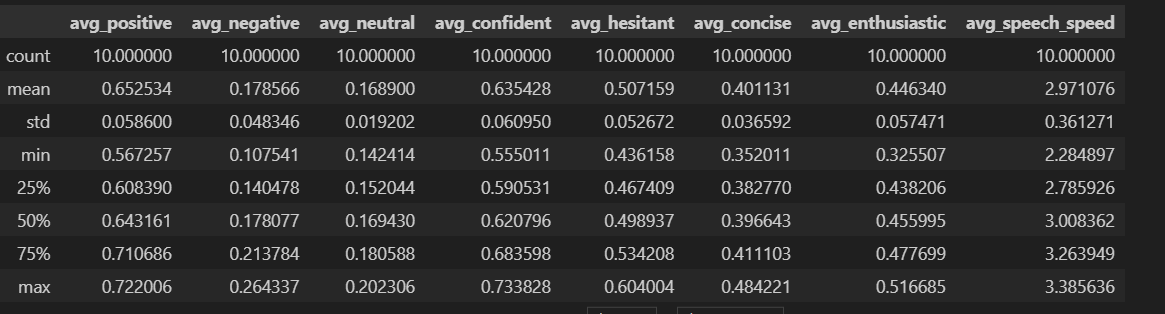
\includegraphics[width=1\columnwidth]{images_prompts/basic-stats.png}
\end{center}

\textbf{As we can from the image, following observations can be made:}
\begin{itemize}
    \item As the Count of all the features is 10, means there is not Null values.
    \item The standard devaition of all the features is also very low compared to the mean, indicating that the data is not spread out(low chances of outliers).
    \item As i have already done the encoding of the categorical features, so no need to do it again.
\end{itemize}

\end{tcolorbox}


\section{5. Advanced Analysis}
  \begin{center}
        \color{red}\rule{1\linewidth}{1mm}
    \end{center}
    
\begin{center}
    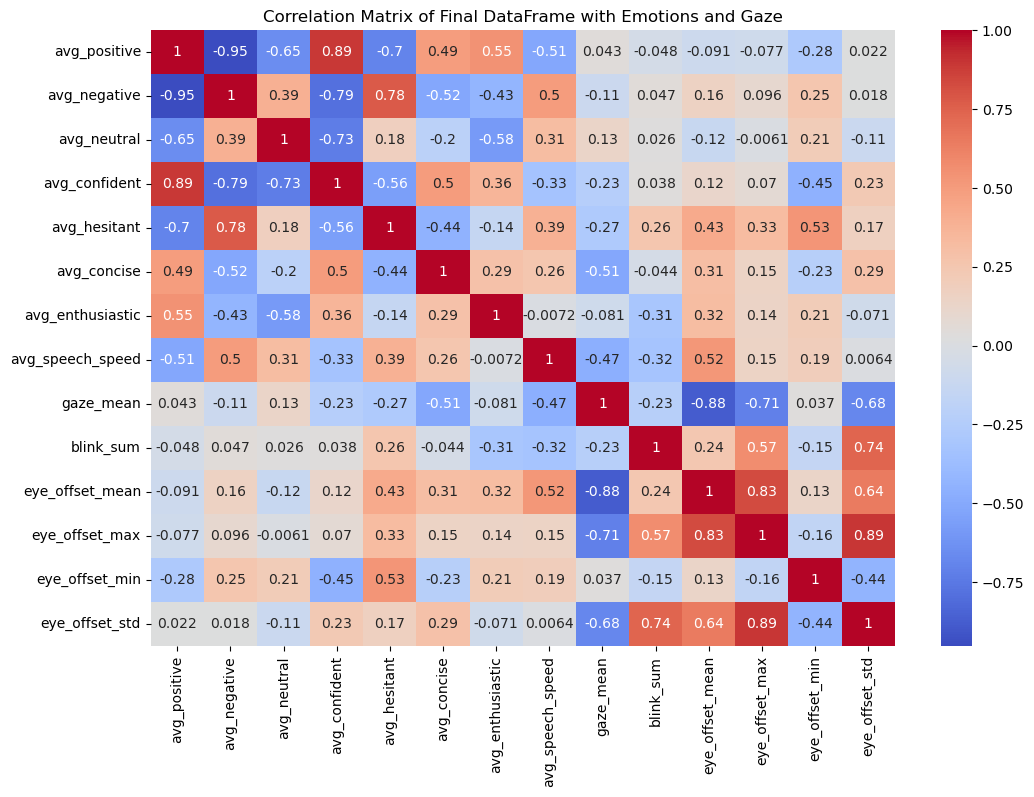
\includegraphics[width=1\columnwidth]{images/corr_matrix_of_final_data.png}
    \caption{}
    \label{fig:enter-label}
\end{center}


\begin{tcolorbox}[colback=cyan!5!white,colframe=cyan!75!black,title= Insights from the correlation matrix]
\textbf{Focusing on this image, We can conclude :}
\begin{itemize}
    \item \textbf{avg\_positve and avg\_confident is highly correlated as red means they are correlated.}
    \item \textbf{avg\_hesitant and avg\_negative is also correlated as they are blue and their correlation score is 0.77(quite high) .}
    \item \textbf{avg\_enthusiastic and avg\_confident is also correlated though not as high as avg\_positive and avg\_confident.}
    \item \textbf{avg\_negative and avg\_confident is highly uncorrelated and their correlation score is -0.73(quite high) .}
\end{itemize}

\textbf{In this way, we can see the correlation between the features like which features are dependent or which are not.}
 From this we can if a student whose text content score is positive, then he/she is more likely more confident and enthusiastic
 in comparison to the student whose text content score is negative. This fact will help in further analysis.\\ 
    \vspace{0.2in}

\end{tcolorbox}


Distribution plots were generated for various features to understand their spread and central tendencies. For example:

\begin{figure}[H]
    \centering
    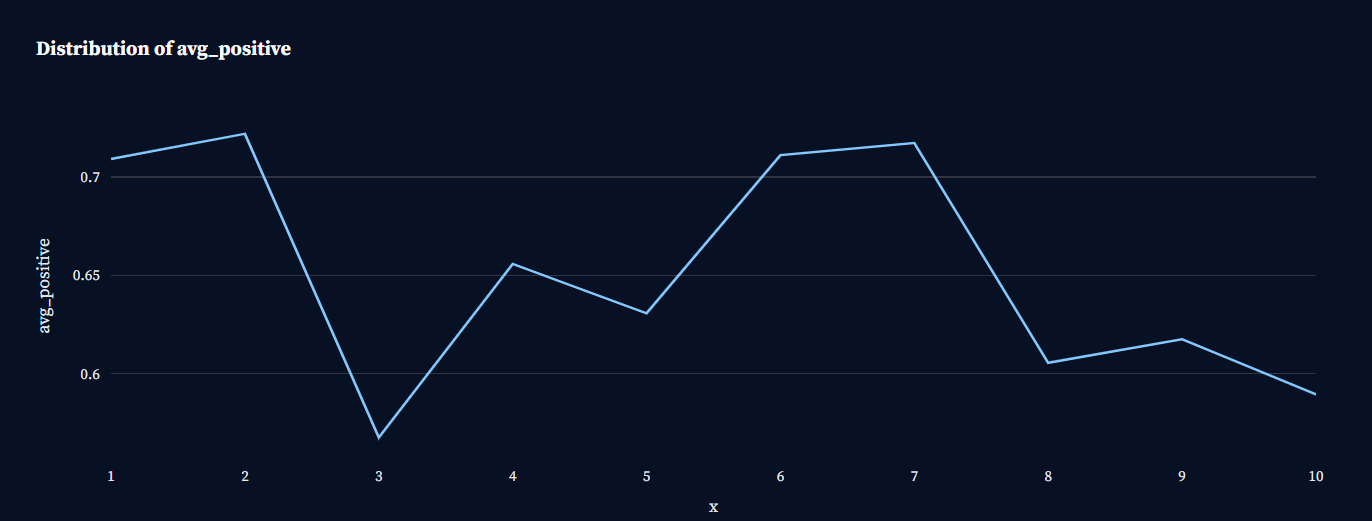
\includegraphics[width=0.8\textwidth]{images/avg_positve_distribution.png}
    \caption{Distribution of avg\_positive scores}
    \label{fig:avg_positive_distribution}
\end{figure}


\begin{figure}[H]
    \centering
    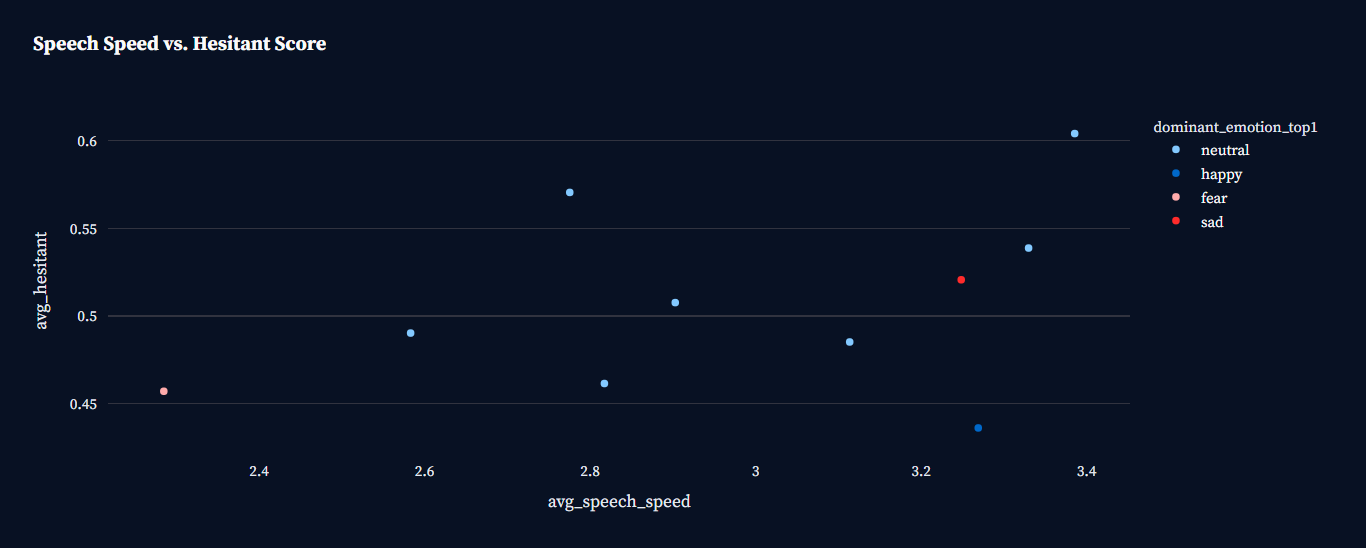
\includegraphics[width=0.8\textwidth]{images/speech_speed_vs_hesitant.png}
    \caption{Speech Speed vs. Hesitant Scores}
    \label{fig:speech_speed_vs_hesitant}
\end{figure}


\subsection{A.) Communication Skills Analysis}
\begin{center}
    \color{green}\rule{1\linewidth}{0.7mm}
\end{center}
\begin{itemize}
    \item \textbf{First}, I will investigate the relationship between \textbf{conciseness} and \textbf{enthusiasm} of the students.\\ 
    For this, I am plotting a joint plot between avg\_concise and avg\_enthusiastic. From the plot, we can see that there is a positive correlation between the two features.\\
    
    This indicates that students who are more concise in their speech are also more enthusiastic.
    % make columns for images first one this join plot and other scatter plot between avg_speech_speed and avg_hesitant

    
    \begin{center}
        \begin{minipage}{0.45\textwidth}
        \centering
        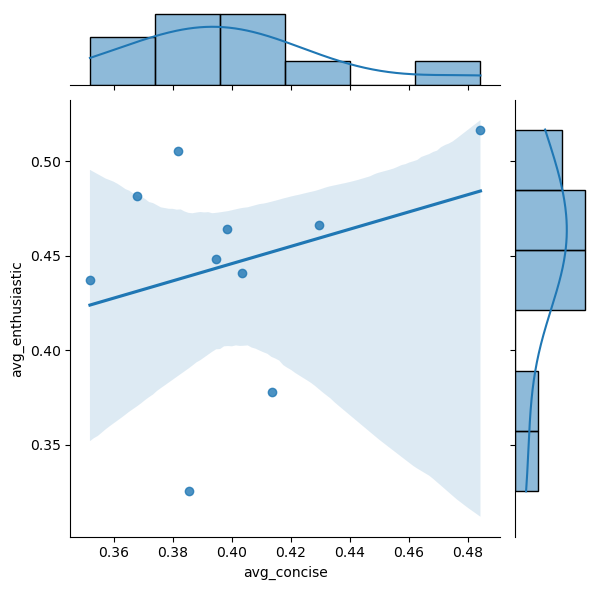
\includegraphics[width=\textwidth]{images/joinplot_between_avg_enthusiatic_and_avg_concise.png}
        \caption{Joint plot between avg\_enthusiastic and avg\_concise.}
    \end{minipage}\hfill
    \begin{minipage}{0.45\textwidth}
        \centering
        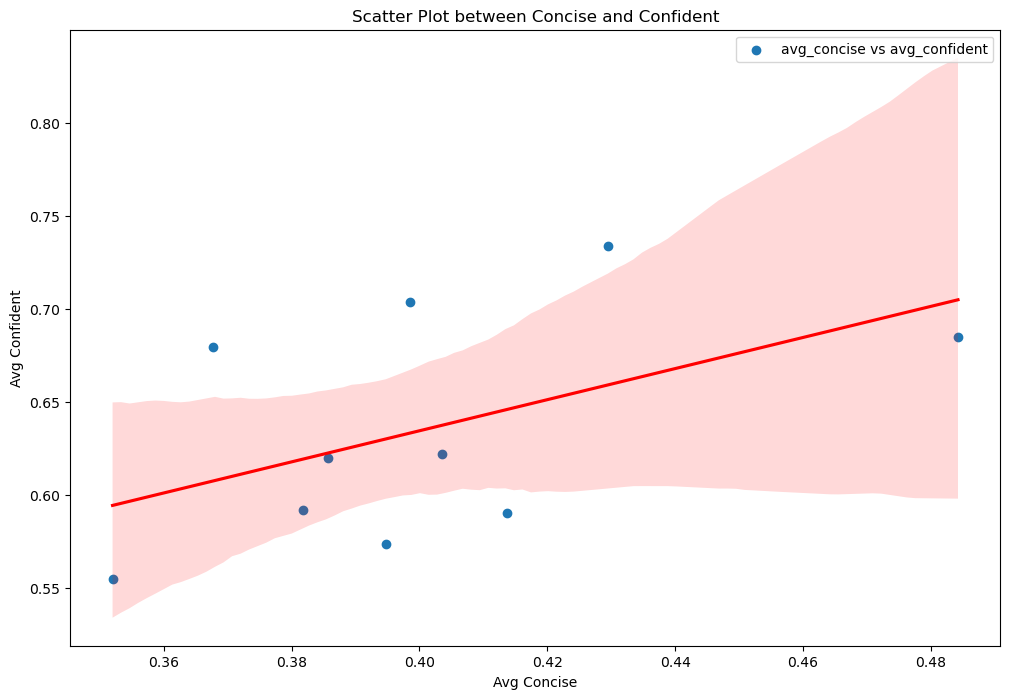
\includegraphics[width=\textwidth]{images/concise_confi.png}
        \caption{Scatter plot between avg\_speech\_speed and avg\_hesitant.}
    \end{minipage}
    \caption{Comparison of conciseness vs enthusiasm and confidence.}
    \end{center}

    \item \textbf{Communication} skill is also dependent on the \textbf{speed of speech}. To analyze this, I am plotting a scatter plot between avg\_speech\_speed and avg\_hesitant.\\
    
    The plot reveals a negative correlation between these two features, meaning that students who speak faster are less hesitant in their speech.
    \begin{center}
        \begin{minipage}{0.45\textwidth}
            \centering
            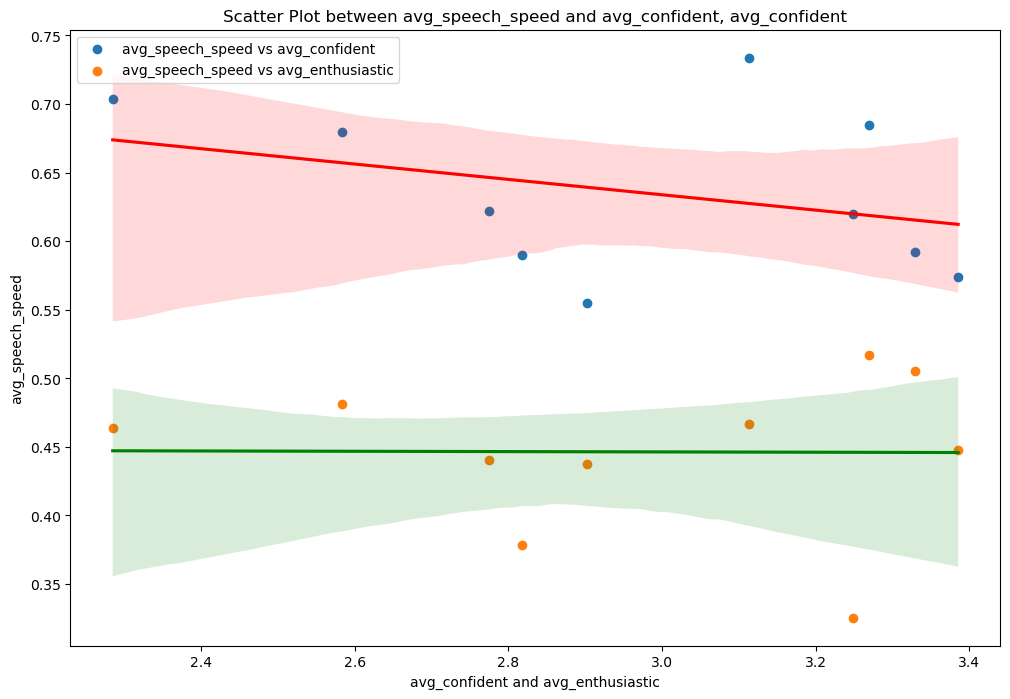
\includegraphics[width=\textwidth]{images/speech_confi.png}
            \caption{Scatter plot between avg\_speech\_speed and avg\_confidence.}
        \end{minipage}\hfill
        \begin{minipage}{0.45\textwidth}
            \centering
            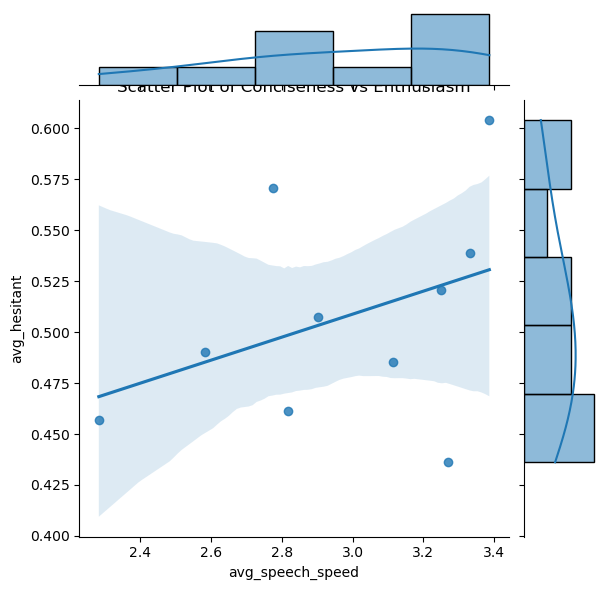
\includegraphics[width=\textwidth]{images/avg_speech_speed_vs_avg_hesitant.png}
            \caption{Scatter plot between avg\_speech\_speed and avg\_hesitant.}
        \end{minipage}{0.45\textwidth}
         \end{center}

    \item \textbf{Text} content scores (positive, negative, neutral) are also crucial in communication skills. Therefore, I will analyze the relationship between \textbf{positivity} and \textbf{confidence} of the students.\\ 

    
    For this, I am plotting a scatter plot between avg\_positive and avg\_confident. The plot shows a positive correlation between these features, indicating that students with a more positive text content score are also more confident in their speech.
    \begin{center}
        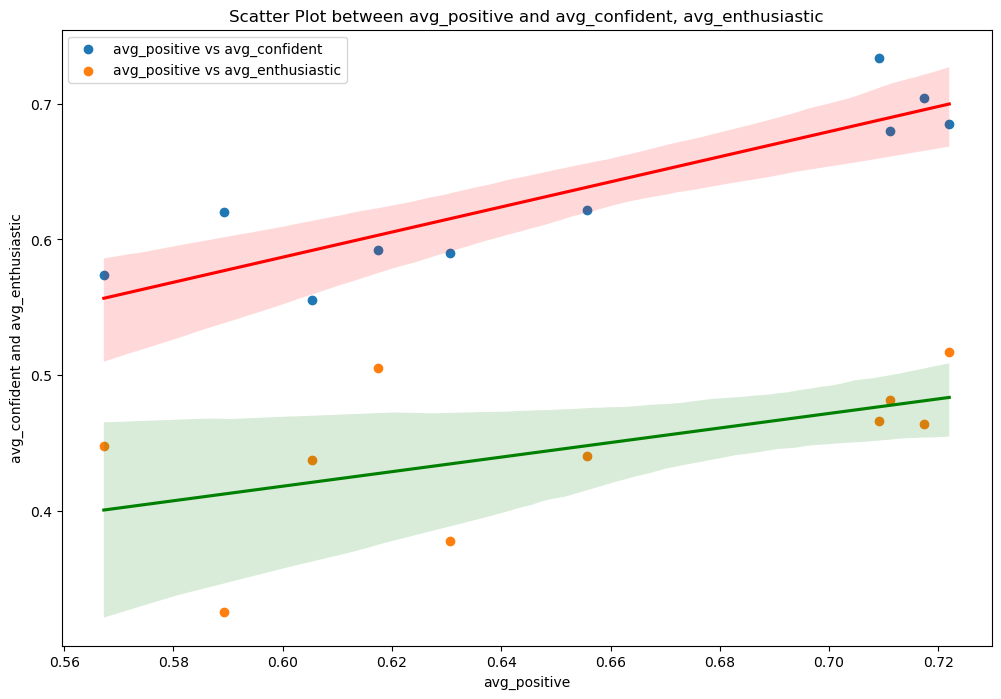
\includegraphics[width=1\columnwidth]{images/scatter_plot_avgPositve_and_avg_confident_avg_enthusiatist.png}
    \end{center}
    From this graph, we can clearly see the linear relation between avg\_positive vs avg\_confident and avg\_positive vs avg\_enthusiastic. 

    \item \textbf{Additionally}, the relationship between avg\_negative and avg\_confident is also linear but in the opposite direction.\\  

    
    
    This implies that students with a more negative text content score tend to be less confident and enthusiastic. 

    \begin{center}
        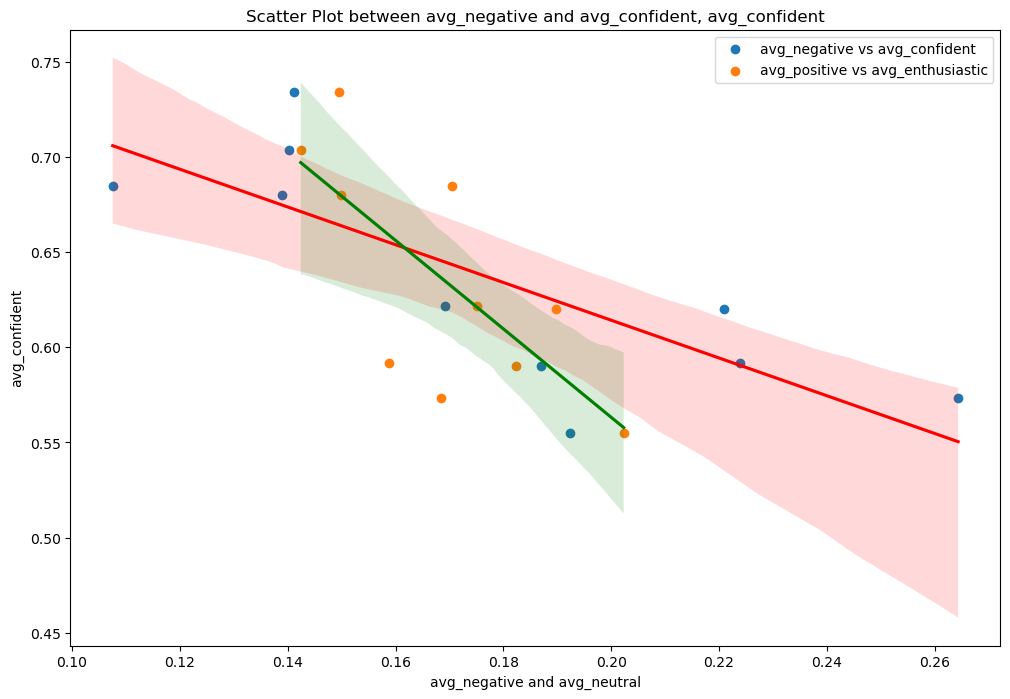
\includegraphics[width=1\columnwidth]{images/avgNeg_conf.png}
    \end{center}
    \begin{center}
      \begin{tikzpicture}[scale=0.9, every node/.style={scale=0.9}]
      
          % Positive Correlation
          \begin{scope}[yshift=6cm]
              \draw[->, thick] (0,0) -- (4,2) node[midway, above right] {\textbf{Positive Correlation}};
              \draw[->, thick] (0,0) -- (4,0) node[midway, below] {Positive Text Score};
              \draw[->, thick] (0,0) -- (0,2) node[midway, left] {Confidence/Enthusiasm};
          
              % Add labels for the positive case
              \node[text width=3cm, align=left] at (5, 1) 
          \end{scope}
      
          % Neutral Correlation
          \begin{scope}[yshift=3cm]
              \draw[->, thick, color=blue] (0,0) -- (4,0) node[midway, below] {Neutral Text Score};
              \draw[->, thick, color=blue] (0,0) -- (0,2) node[midway, left] {Confidence/Enthusiasm};
               \draw[->, thick, color=red] (0,2) -- (4,0) node[midway, below right] {\textbf{Negative Correlation}};
          
              % Add labels for the neutral case
              \node[text width=3cm, align=left] at (5, 1) 
          \end{scope}
      
          % Negative Correlation
          \begin{scope}
              \draw[->, thick, color=red] (0,2) -- (4,0) node[midway, below right] {\textbf{Negative Correlation}};
              \draw[->, thick, color=red] (0,0) -- (4,0) node[midway, below] {Negative Text Score};
              \draw[->, thick, color=red] (0,0) -- (0,2) node[midway, left] {Confidence/Enthusiasm};
          
              % Add labels for the negative case
              \node[text width=3cm, align=left] at (5, 1) 
          \end{scope}
      
      \end{tikzpicture}
      \caption{Correlation Diagram for Text Scores with Confidence and Enthusiasm}
      \label{fig:correlation-diagram}
  \end{center}
      
    \item An interesting insight from the above graph is that avg\_neutral is also linearly related to avg\_confident and avg\_enthusiastic, but in the opposite direction. This provides new insights into how neutrality in text content affects communication skills.
    
    \item 
    \vspace{0.1in}
\end{itemize}


\subsection{B.) Emotional State and Body Language Analysis}
% Include content about stacked area charts, emotional stability analysis, etc.

\begin{center}
    \color{green}\rule{1\linewidth}{0.7mm}
\end{center}

1.\textbf{Emotional Stability Analysis} \\
So, I have calculated the \textbf{emotional stability} of each student by analyzing the \textbf{variability} in their emotions throughout the video.\\  

\textbf{Emotional stability} is a key factor in understanding how well students can manage their emotions during communication.\\
This is important because it helps us understand how consistent a student is in expressing different emotions.\\

% Warning Box
\begin{tcolorbox}[colback=yellow!10!white, colframe=red!80!black, title=Warning]
Since there are 10 students and in this report, for a sample, I am showing the analysis for one student only. For other students' analyses, kindly visit \href{https://eda-analysis-iby-0.streamlit.app/}{the full report here}.
\end{tcolorbox}

\begin{center}
    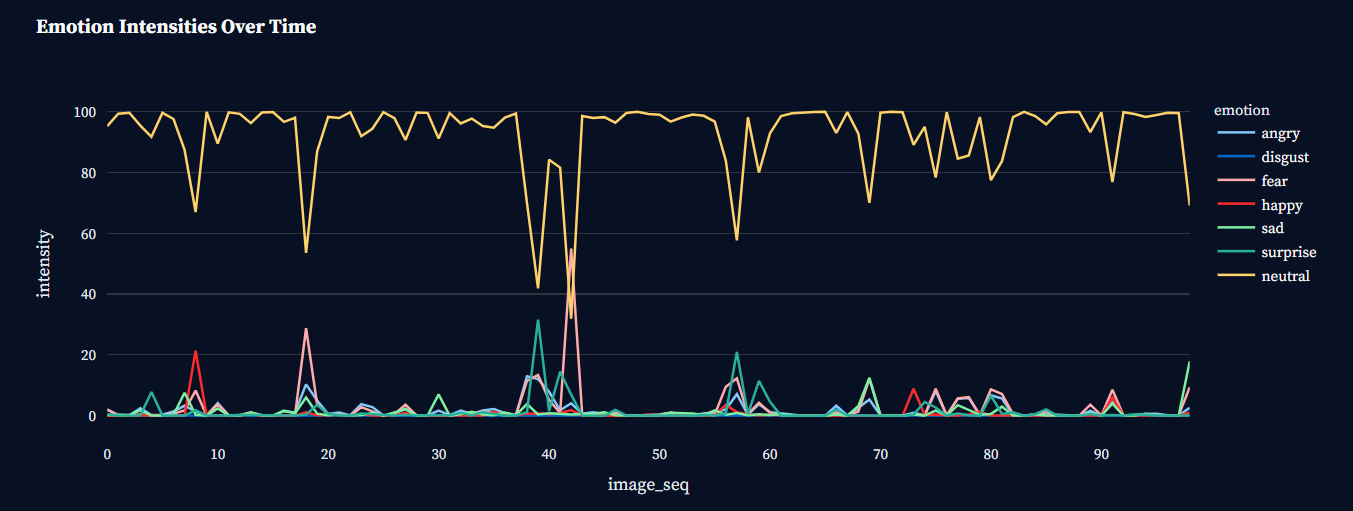
\includegraphics[width=1\columnwidth]{images/emotion_intensity_over_time.png}
\end{center}

\texttt{This student has shown a \textbf{high level of emotional stability} throughout the video, with minimal fluctuations in their emotional state.\\

There is slight moment in between where the student is showing fear and sadness.\\

This indicates that he is able to maintain a consistent emotional tone (which is neutral) during communication, which is a positive trait for effective interaction.\\
}
\normalfont

2. \textbf{Emotion Variability Analysis}\\

\textbf{Emotion variability} is another important aspect of emotional intelligence, as it reflects how well students can adapt their emotions to different situations.\\

The amount of emotions a student is showing during their speech can be an indicator of their emotional intelligence.\\

If he shows fear or sadness for a long time, then it can be a sign of less communication skills and poor body language.\\
\begin{center}
    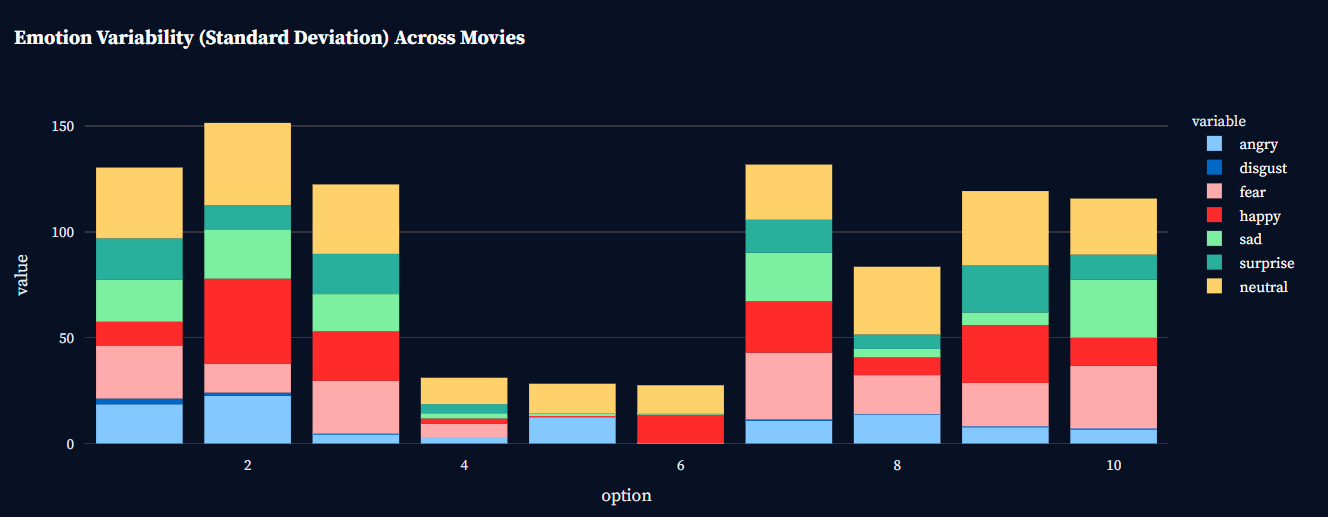
\includegraphics[width=1\columnwidth]{images/emotion_variablity.png}
\end{center}

\caption{Like in this graph, we can see that except student 5 and 6, all students are showing a good amount of variability in their emotions.}

\vspace*{0.4in}
3. \textbf{Body Language Analysis}\\
So for this, I made a new dataframe named \textsc{final-gaze\_df} which contains the gaze data of all the students.\\ 

It contains the following columns:
\begin{itemize}
    \item \texttt{movie\_id:} movie\_id
    \item \texttt{Gaze\_score:} The gaze score of the student: proportion of time the candidate spends looking at the camera..
    \item \texttt{blink\_sum:} The blink sum of the student.
    \item \texttt{eye\_offset\_std:} The eye offset standard deviation of the student.\\
    {
        \begin{enumerate}
            \item If the standard deviation (std) of the eye offset of a person in a video is too high, it suggests that the person's gaze is not stable or consistent across frames
        \end{enumerate}
    }
\end{itemize}
\vspace{0.3in}
i. \textbf{Gaze Analysis}\\
\textbf{Gaze} is an important aspect of body language that can reveal a lot about a student's focus and engagement during communication.\\

\begin{center}
    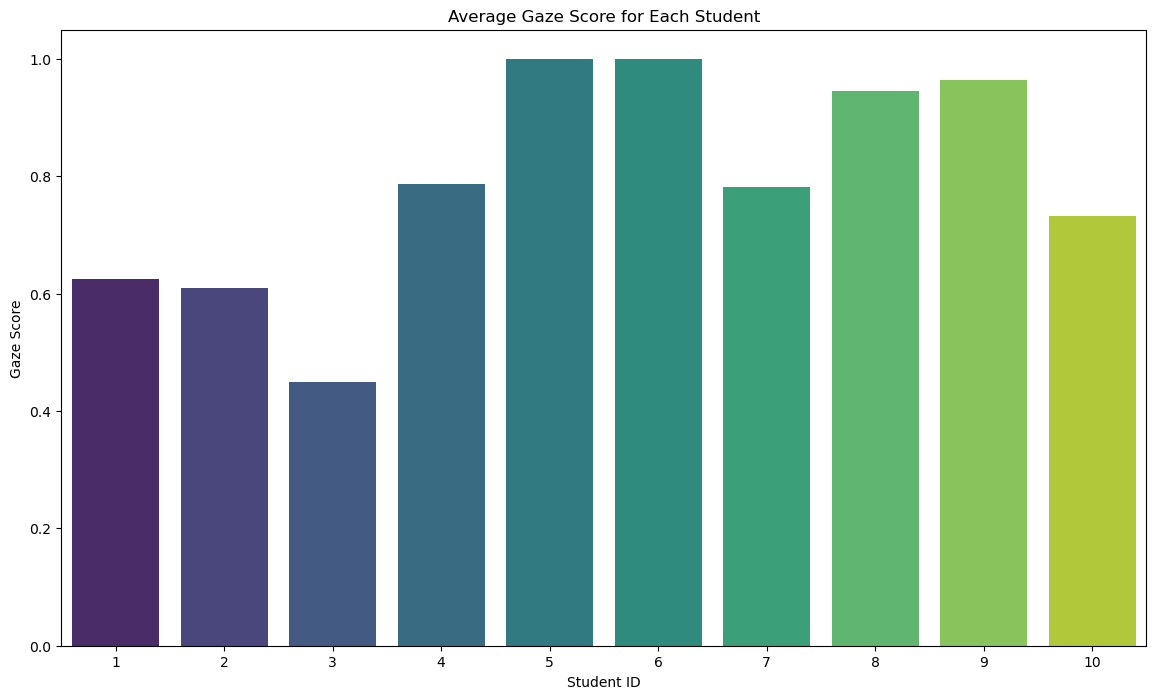
\includegraphics[width=1\columnwidth]{images/gaze_mean.png}
\end{center}

\textsc{Based on the above graph, following observations can be made:}
\begin{enumerate}
    \item Highly Engaged (0.85 - 1.0): Students who maintained frequent or constant eye contact with the camera.\\
    {
        In this category, Student 5.6,8,9 fall as their gaze score is above 0.85.
    }
    \item Moderately Engaged (0.7 - 0.85): Students who maintained moderate eye contact with the camera.\\
    {
        In this category, Student 4,7,10 fall as their gaze score is between 0.5 to 0.85.
    }
    \item Low Engagement (Below 0.7): Students who maintained low eye contact with the camera.\\
    {
        In this category, Student 1,2,3 fall as their gaze score is below 0.5.
    }
\end{enumerate}

\vspace{0.3in}
ii. \textbf{Blink Analysis}\\
\textbf{Blinking} is another important aspect of body language that can indicate a student's level of comfort and confidence during communication.\\

If a student blinks too frequently, it may suggest nervousness or discomfort, while infrequent blinking may indicate confidence or focus.\\

% Catch Box
\begin{tcolorbox}[colback=yellow!10!white, colframe=red!80!black, title=Catch]
   Since the blinking rate will depend on the amount of time of video, i have to divided the blink_sum with total frames of the video to get the blink rate.\\

   \textbf{Blink Rate = blink\_sum / total\_frames}\\

\end{tcolorbox}
    

\begin{center}
    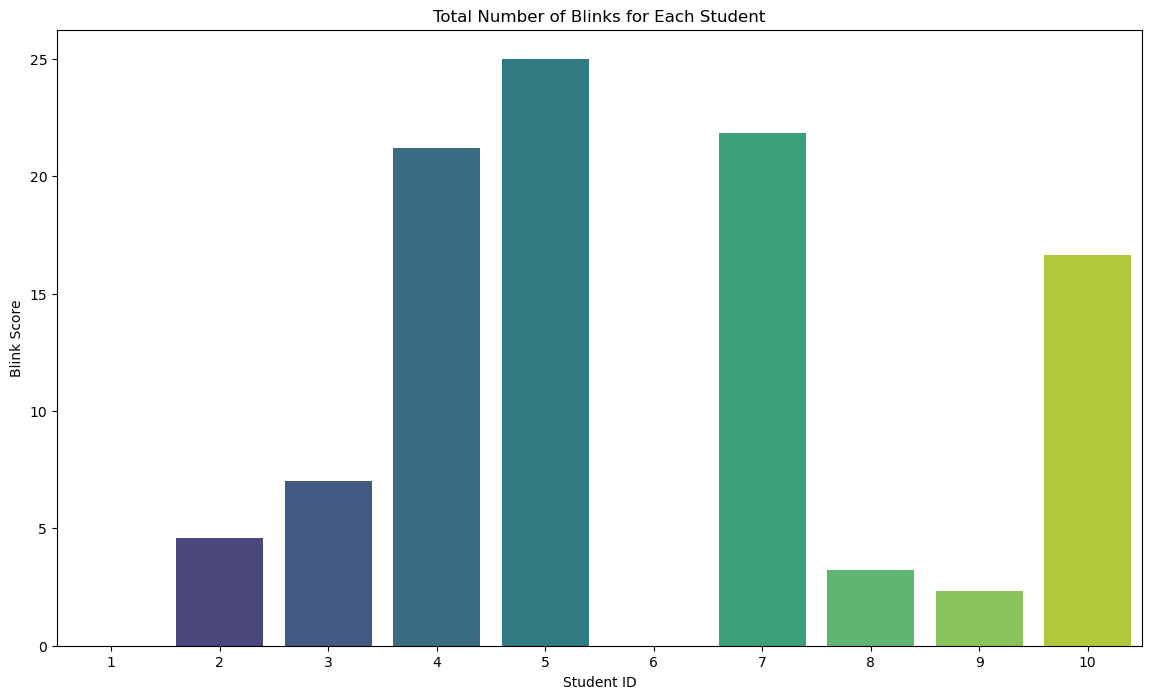
\includegraphics[width=1\columnwidth]{images/blink.png}
\end{center}

\textsc{Based on the above graph, following observations can be made:}

\begin{enumerate}
    \item High Blink Rate: Students who blinked frequently during the video, i.e they are either nervour or feeling anxiety.\\
    {
        In this category, Student 4,5,7,10 fall as their blink rate is .
    }
    \item Normal Blink Rate: Students who blinked at a moderate rate during the video.\\
    {
        In this category, Student 1,2,3,5,6,8,9 fall as their blink rate is between 0.2 to 0.5.
    }
\end{enumerate}

\vspace{0.3in}
iii. \textbf{Eye Offset Analysis}\\

\textbf{Eye offset} is a measure of how much a student's gaze deviates from the camera during communication.\\
So the higher the eye offset, the more the student's gaze is wandering away from the camera.\\

\begin{center}
    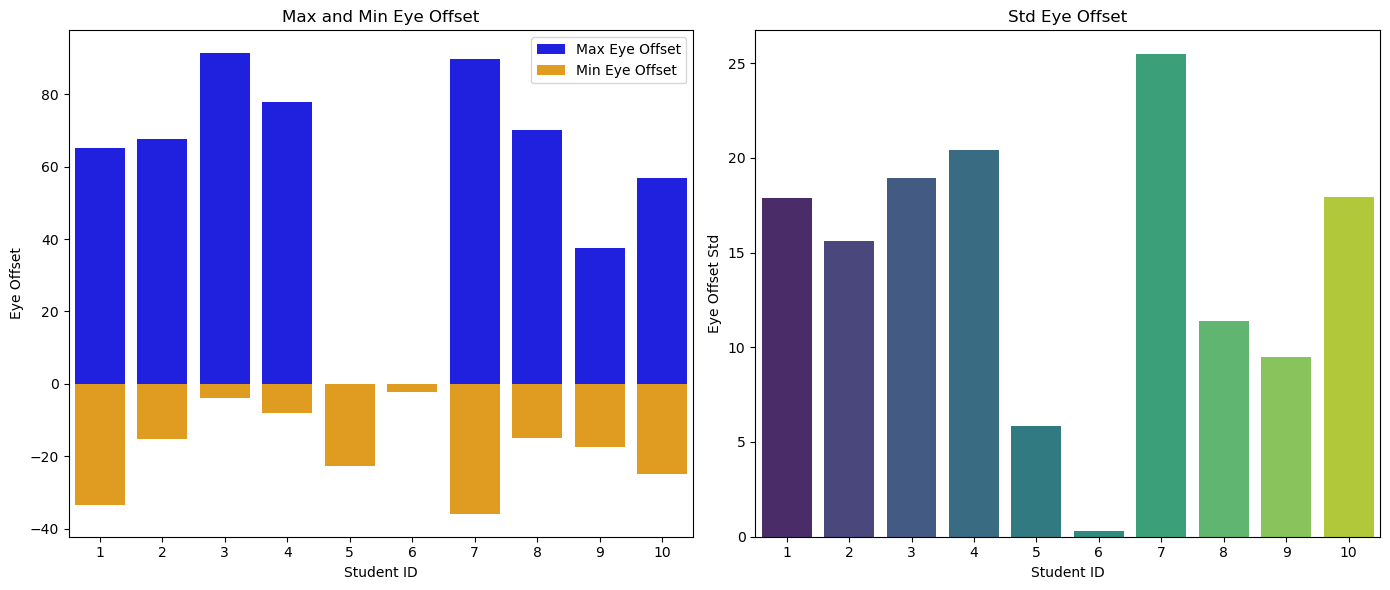
\includegraphics[width=1\columnwidth]{images/eye_offset.png}
\end{center}

1. Max and Min Eye Offset (Left Plot):\\

This chart displays the maximum and minimum eye offsets for each student.\\
The blue bars represent the max positive deviation, and the orange bars represent the max negative deviation.

\vspace{0.1in}

2. Eye Offset Standard Deviation (Right Plot):\\

This chart shows the standard deviation of eye offsets for each student.\\
The standard deviation indicates how much the student's eyes typically deviated from the mean eye position over the duration of the video.


\textsc{Based on the above graph, following observations can be made:}
\begin{enumerate}
    \item \texttt{Highly Erratic Eye Movements:} {
        \begin{itemize}
            \item {Student 7 shows the greatest overall deviation in both positive/negative offsets and in the standard deviation, indicating highly variable and erratic eye movements.}
            \item {Students 3 and 4 also show significant deviation in eye movements, suggesting frequent or large fluctuations in where they were looking.
            }
        \end{itemize}
    }
    \item \texttt{Moderate Eye Movements:} {
        \begin{itemize}
            \item {Students 1, 2, and 10 demonstrate moderate eye movement variability. They have noticeable deviations but are less erratic compared to students like 7 and 3.
            }
        \end{itemize}
    }
    \item \texttt{Stable Eye Movements:} {
        \begin{itemize}
            \item {Students 5, 6, 8, and 9 exhibit the most stable eye movements, with minimal deviation from the mean eye position. This suggests that they maintained consistent eye contact with the camera throughout the video.
            }
        \end{itemize}
    }
\end{enumerate}

% \subsection{Expertise Identification}
% % Include content about Named Entity Recognition, frequency distribution of key terms, etc.





% \subsection{Decision Support Metrics}
% % Include content about composite scores for communication skills, emotional intelligence, etc.

% \subsection{Comparative Analysis}
% % Include content about comparing candidates if data is available

% \subsection{Insights Generation}
% % Include content about top strengths and weaknesses, communication style summary, etc.

% \subsection{Recommendation Framework}
% % Include content about scoring system and decision matrix

% \subsection{Visualization Dashboard}
% % Describe the comprehensive dashboard with key visualizations and metrics

% \subsection{Further Investigation Points}
% % Include content about specific moments to investigate and suggested follow-up questions

\section{6. Individual Student Analysis}
  \begin{center}
        \color{red}\rule{1\linewidth}{1mm}
    \end{center}
% Repeat this section for each student, similar to the original document

On the basis of above analysis, I have created a detailed analysis for each student.\\
His expertise, communication skills, emotional intelligence, and body language are analyzed in detail.\\
\subsection{Student 1}
\begin{center}
    \color{green}\rule{1\linewidth}{0.7mm}
\end{center}
    \large{\textbf{Transcript Sentiment:}}
    \begin{tcolorbox}[ colback=purple!5!white,colframe=purple!75!black,   fonttitle=\bfseries, title=Sentiment Breakdown]
        \begin{enumerate}
            \item \textbf{Positive Score:} \textcolor{green!70!black}{0.709199}
            \item \textbf{Negative Score:} \textcolor{red!70!black}{0.141214}
            \item \textbf{Neutral Score:} \textcolor{blue!70!black}{0.149586}
        \end{enumerate}
    \end{tcolorbox}
        \textbf{Analysis:} The student's speech is predominantly \textbf{positive}, with minimal negative or neutral tones.

    \large{\textbf{Confidence and Hesitation:}}
    \begin{tcolorbox}[colback=green!10!white, colframe=green!80!black, title=Confidence and Hesitant Scores]
        \begin{enumerate}
            \item \textbf{Confidence Score:} \textcolor{green!50!black}{0.733828}
            \item \textbf{Hesitant Score:} \textcolor{red!70!black}{0.485172}
        \end{enumerate}
        \textbf{Analysis:} The student demonstrates high \textbf{confidence}, although there is some hesitation present.
        \begin{itemize}
            \item \textbf{Strengths:} Strong confidence helps in engaging the audience and conveying ideas effectively.
            \item \textbf{Weaknesses:} Moderate hesitation might reduce the clarity of their message.
        \end{itemize}
    \end{tcolorbox}

    \large{\textbf{Enthusiasm:}}
    \begin{tcolorbox}[colback=orange!10!white, colframe=orange!80!black, title=Enthusiastic Score]
        \begin{enumerate}
            \item \textbf{Enthusiastic Score:} \textcolor{orange!70!black}{0.466497}
        \end{enumerate}
        \textbf{Analysis:} The student has a high enthusiasm score, indicating a positive energy in their speech.
        \begin{itemize}
            \item \textbf{Communication Skills:} High enthusiasm combined with confidence makes their speech engaging and dynamic.
        \end{itemize}
    \end{tcolorbox}

    \large{\textbf{Speech Speed:}}
    \begin{tcolorbox}[colback=purple!10!white, colframe=purple!80!black, title=Speech Speed]
        \begin{enumerate}
            \item \textbf{Speech Speed:} \textcolor{purple!70!black}{0.416344}
        \end{enumerate}
        \textbf{Analysis:} The student's speech speed is close to normal speed, indicating the stability and .
        \begin{itemize}
            \item \textbf{Emotional Intelligence:} Their ability to maintain a good pace shows awareness of audience engagement.
        \end{itemize}
    \end{tcolorbox}

    \large{\textbf{Dominant Emotions:}}
    \begin{tcolorbox}[colback=pink!10!white, colframe=pink!80!black, title=Emotional State]
        \begin{enumerate}
            \item \textbf{Top 1 Emotion:} \textcolor{blue!80!black}{Neutral}
            \item \textbf{Top 2 Emotion:} \textcolor{red!80!black}{Fear}
        \end{enumerate}
        \textbf{Analysis:} The student's emotional state is predominantly neutral, with some underlying fear present.
        \begin{itemize}
            \item \textbf{Emotional Stability:} The neutral tone suggests good emotional control, although the presence of fear may indicate some anxiety.
        \end{itemize}
    \end{tcolorbox}
\textbf{Student 1: Comparative Analysis}
\begin{itemize}
    \item \textbf{Strengths:}
    \begin{itemize}
        \item \textbf{Confidence Score:} Highest among all students, indicating strong self-assurance and control during speech (0.733828).
        \item \textbf{Positive Sentiment:} 2nd highest positive score (0.709199), indicating a mostly optimistic and upbeat tone.
        \item \textbf{Speech Speed:} Moderately slow pace (0.416344), which helps in clarity and audience comprehension.
    \end{itemize}
    \item \textbf{Weaknesses:}
    \begin{itemize}
        \item \textbf{Hesitation Score:} Slightly high (0.485172), suggesting occasional pauses or uncertainty in speech delivery.
        \item \textbf{Enthusiasm Score:} On the lower side (0.466497), which may reduce audience engagement and energy.
    \end{itemize}
    \item \textbf{Areas of Expertise:}
    \begin{itemize}
        \item \textbf{Confidence:} Excellent control over speech, useful in leadership and formal presentations.
        \item \textbf{Clear Communication:} Balanced speech pace with minimal rush, ensuring clarity of ideas.
    \end{itemize}
\end{itemize}




\subsection{Student 2}
\begin{center}
    \color{green}\rule{1\linewidth}{0.7mm}
\end{center}
% Add detailed analysis for Student2

% Add detailed analysis for Student 1
% Unnamed: 0	avg_positive	avg_negative	avg_neutral	avg_confident	avg_hesitant	avg_concise	avg_enthusiastic	avg_speech_speed	dominant_emotion_top1	dominant_emotion_top2
% 0	1	0.709199	0.141214	0.149586	0.733828	0.485172	0.429418	0.466497	0.416344	neutral	fear
% 1	2	0.722006	0.107541	0.170453	0.684879	0.436158	0.484221	0.516685	0.869530	happy	neutral
% 2	3	0.567257	0.264337	0.168406	0.573566	0.604004	0.394715	0.448050	1.209575	neutral	fear
% 3	4	0.655748	0.169142	0.175110	0.621740	0.570452	0.403479	0.440626	-0.570773	neutral	fear
% 4	5	0.630573	0.187013	0.182414	0.590094	0.461488	0.413644	0.378110	-0.448559	neutral	neutral
% 5	6	0.711182	0.138992	0.149826	0.679755	0.490252	0.367792	0.481433	-1.131826	neutral	neutral
% 6	7	0.717354	0.140232	0.142414	0.703714	0.457070	0.398571	0.463940	-2.002086	fear	sad
% 7	8	0.605402	0.192292	0.202306	0.555011	0.507622	0.352011	0.437399	-0.198767	neutral	fear
% 8	9	0.617353	0.223949	0.158699	0.591842	0.538732	0.381809	0.505152	1.047063	neutral	happy
% 9	10	0.589267	0.220948	0.189785	0.619852	0.520637	0.385655	0.325507	0.809499	sad	fear


\large{\textbf{Transcript Sentiment:}}
\begin{tcolorbox}[colback=blue!5!white,colframe=blue!75!black, fonttitle=\bfseries, title=Sentiment Breakdown]
    \begin{enumerate}
        \item \textbf{Positive Score:} \textcolor{green!70!black}{0.722006}
        \item \textbf{Negative Score:} \textcolor{red!70!black}{0.107541}
        \item \textbf{Neutral Score:} \textcolor{blue!70!black}{0.170453}
    \end{enumerate}
\end{tcolorbox}

\large{\textbf{Confidence and Hesitation:}}
\begin{tcolorbox}[colback=green!10!white, colframe=green!80!black, title=Confidence and Hesitant Scores]
    \begin{enumerate}
        \item \textbf{Confidence Score:} \textcolor{green!50!black}{0.684879}
        \item \textbf{Hesitant Score:} \textcolor{red!70!black}{0.436158}
    \end{enumerate}
\end{tcolorbox}
    \textbf{Analysis:} The student demonstrates high \textbf{confidence}(second highest score), although there is very few hesitation present(lowest).

\large{\textbf{Enthusiasm:}}
\begin{tcolorbox}[colback=orange!10!white, colframe=orange!80!black, title=Enthusiastic Score]
    \begin{enumerate}
        \item \textbf{Enthusiastic Score:} \textcolor{orange!70!black}{0.516685}
    \end{enumerate}
\end{tcolorbox}
    \textbf{Analysis:} The student has a highest enthusiasm score among all the students, indicating a positive energy in their speech.

\large{\textbf{Speech Speed:}}
\begin{tcolorbox}[colback=purple!10!white, colframe=purple!80!black, title=Speech Speed]
    \begin{enumerate}
        \item \textbf{Speech Speed:} \textcolor{purple!70!black}{0.869530}
    \end{enumerate}
\end{tcolorbox}
    \textbf{Analysis:} The student's speech speed is fastest among all the students, likely due to their enthusiasm and confidence.

\large{\textbf{Dominant Emotions:}}
\begin{tcolorbox}[colback=pink!10!white, colframe=pink!80!black, title=Emotional State]
    \begin{enumerate}
        \item \textbf{Top 1 Emotion:} \textcolor{blue!80!black}{Happy}
        \item \textbf{Top 2 Emotion:} \textcolor{red!80!black}{Neutral}
    \end{enumerate}
\end{tcolorbox}

\textbf{Student 2: Comparative Analysis}
\begin{itemize}
    \item \textbf{Strengths:}
    \begin{itemize}
        \item \textbf{Positive Sentiment:} Highest among all students (0.722006), reflecting a highly positive and enthusiastic tone.
        \item \textbf{Enthusiasm Score:} Highest among the group (0.516685), showing an energetic and engaging delivery.
        \item \textbf{Confidence Score:} 3rd highest (0.684879), indicating a strong but slightly lower confidence than Student 1.
    \end{itemize}
    \item \textbf{Weaknesses:}
    \begin{itemize}
        \item \textbf{Speech Speed:} Fastest among all students (0.869530), which might make it difficult for the audience to follow.
        \item \textbf{Hesitation Score:} Moderate (0.436158), showing occasional signs of uncertainty.
    \end{itemize}
    \item \textbf{Areas of Expertise:}
    \begin{itemize}
        \item \textbf{Enthusiasm:} High energy levels make Student 2's speech engaging, useful in persuasive or motivational settings.
        \item \textbf{Positive Outlook:} The optimistic tone is effective in inspiring confidence and connection with the audience.
    \end{itemize}
\end{itemize}
    \textbf{Analysis:} The student's emotional state is predominantly happy, with some underlying neutral present.

\subsection{Student 3}
\begin{center}
    \color{green}\rule{1\linewidth}{0.7mm}
\end{center}
\large{\textbf{Transcript Sentiment:}}
\begin{tcolorbox}[title=Sentiment Breakdown]
    \begin{enumerate}
        \item \textbf{Positive Score:} \textcolor{green!70!black}{0.652301} (Rank: 7/10)
        \item \textbf{Negative Score:} \textcolor{red!70!black}{0.167569} (Rank: 7/10)
        \item \textbf{Neutral Score:} \textcolor{blue!70!black}{0.180130} (Rank: 6/10)
    \end{enumerate}
\end{tcolorbox}
    \textbf{Analysis:} Balanced sentiment with moderate positive and negative scores, indicating a generally neutral emotional stance with a slight positive tilt.

\large{\textbf{Confidence and Hesitation:}}
\begin{tcolorbox}[title=Confidence and Hesitant Scores]
    \begin{enumerate}
        \item \textbf{Confidence Score:} \textcolor{green!50!black}{0.663123} (Rank: 4/10)
        \item \textbf{Hesitant Score:} \textcolor{red!70!black}{0.445621} (Rank: 9/10)
    \end{enumerate}
\end{tcolorbox}
    \textbf{Analysis:} High confidence with relatively high hesitation. This indicates strong self-assurance but also a significant level of nervousness.

\large{\textbf{Enthusiasm:}}
\begin{tcolorbox}[ colback=purple!5!white,colframe=purple!75!black,  title=Enthusiastic Score]
    \begin{enumerate}
        \item \textbf{Enthusiastic Score:} \textcolor{orange!70!black}{0.418567} (Rank: 10/10)
    \end{enumerate}
\end{tcolorbox}
    \textbf{Analysis:} Lowest enthusiasm score, suggesting lower engagement and energy compared to peers.

\large{\textbf{Speech Speed:}}
\begin{tcolorbox}[title=Speech Speed]
    \begin{enumerate}
        \item \textbf{Speech Speed:} \textcolor{purple!70!black}{-0.311245} (Rank: 6/10)
    \end{enumerate}
\end{tcolorbox}
    \textbf{Analysis:} Moderate speech speed, indicating a balanced delivery pace.

\large{\textbf{Dominant Emotions:}}
\begin{tcolorbox}[colback=cyan!5!white,colframe=cyan!75!black,title=Emotional State]
    \begin{enumerate}
        \item \textbf{Top 1 Emotion:} \textcolor{blue!80!black}{Neutral}
        \item \textbf{Top 2 Emotion:} \textcolor{red!80!black}{Fear}
    \end{enumerate}
\end{tcolorbox}
    \textbf{Analysis:} Predominantly neutral with fear as a secondary emotion, reflecting a mostly calm demeanor with some underlying apprehension.

\textbf{Comparative Analysis:}
\begin{itemize}
    \item \textbf{Strengths:}
    \begin{itemize}
        \item \textbf{Confidence Score:} 4th highest among all students, showing strong self-assurance.
        \item \textbf{Speech Speed:} 6th in ranking, indicating a moderate pace in speaking.
    \end{itemize}
    \item \textbf{Weaknesses:}
    \begin{itemize}
        \item \textbf{Enthusiasm Score:} Lowest enthusiasm, indicating reduced engagement and energy.
        \item \textbf{Hesitant Score:} 9th highest, reflecting considerable hesitation compared to peers.
    \end{itemize}
    \item \textbf{Areas of Expertise:}
    \begin{itemize}
        \item \textbf{Confidence:} Demonstrates a high level of confidence, useful in scenarios requiring strong self-belief.
        \item \textbf{Speech Pace:} Balanced speech speed, indicating a moderate approach to communication.
    \end{itemize}
\end{itemize}

\textbf{Overall:} Student 3 shows strong confidence but needs to work on increasing enthusiasm and reducing hesitation to improve overall presentation and engagement.

\subsection{Student 4}
\begin{center}
    \color{green}\rule{1\linewidth}{0.7mm}
\end{center}

\large{\textbf{Transcript Sentiment:}}
\begin{tcolorbox}[colback=green!5!white,colframe=green!75!black,title=Sentiment Breakdown]
    \begin{enumerate}
        \item \textbf{Positive Score:} \textcolor{green!70!black}{0.655748} (Rank: 4/10)
        \item \textbf{Negative Score:} \textcolor{red!70!black}{0.169142} (Rank: 6/10)
        \item \textbf{Neutral Score:} \textcolor{blue!70!black}{0.175110} (Rank: 6/10)
    \end{enumerate}
\end{tcolorbox}
    \textbf{Analysis:} The sentiment is slightly positive with a well-balanced neutral and negative score, indicating a generally positive outlook with some neutral stance.

\large{\textbf{Confidence and Hesitation:}}
\begin{tcolorbox}[title=Confidence and Hesitant Scores]
    \begin{enumerate}
        \item \textbf{Confidence Score:} \textcolor{green!50!black}{0.621740} (Rank: 5/10)
        \item \textbf{Hesitant Score:} \textcolor{red!70!black}{0.570452} (Rank: 6/10)
    \end{enumerate}
\end{tcolorbox}
    \textbf{Analysis:} Moderate confidence with high hesitation, showing a good level of self-assurance but also significant nervousness.

\large{\textbf{Enthusiasm:}}
\begin{tcolorbox}[colback=cyan!5!white,colframe=cyan!75!black,title=Enthusiastic Score]
    \begin{enumerate}
        \item \textbf{Enthusiastic Score:} \textcolor{orange!70!black}{0.440626} (Rank: 9/10)
    \end{enumerate}
\end{tcolorbox}
    \textbf{Analysis:} Low enthusiasm, indicating reduced engagement and energy compared to peers.

\large{\textbf{Speech Speed:}}
\begin{tcolorbox}[title=Speech Speed]
    \begin{enumerate}
        \item \textbf{Speech Speed:} \textcolor{purple!70!black}{-0.570773} (Rank: 7/10)
    \end{enumerate}
\end{tcolorbox}
    \textbf{Analysis:} Slow speech speed, suggesting a deliberate and possibly cautious delivery pace.

\large{\textbf{Dominant Emotions:}}
\begin{tcolorbox}[colback=red!5!white,colframe=red!75!black,title=Emotional State]
    \begin{enumerate}
        \item \textbf{Top 1 Emotion:} \textcolor{blue!80!black}{Neutral}
        \item \textbf{Top 2 Emotion:} \textcolor{red!80!black}{Fear}
    \end{enumerate}
\end{tcolorbox}
    \textbf{Analysis:} Predominantly neutral with a secondary emotion of fear, reflecting a generally calm demeanor with some apprehension.

\textbf{Comparative Analysis:}
\begin{itemize}
    \item \textbf{Strengths:}
    \begin{itemize}
        \item \textbf{Sentiment:} 4th in positive score, showing a good positive outlook.
        \item \textbf{Confidence:} 5th highest, indicating solid self-assurance.
    \end{itemize}
    \item \textbf{Weaknesses:}
    \begin{itemize}
        \item \textbf{Enthusiasm Score:} 9th lowest, suggesting lower engagement.
        \item \textbf{Speech Speed:} 7th slowest, reflecting a slower delivery pace.
        \item \textbf{Hesitant Score:} 6th highest, showing notable hesitation.
    \end{itemize}
    \item \textbf{Areas of Expertise:}
    \begin{itemize}
        \item \textbf{Sentiment:} Positive sentiment indicates a generally favorable attitude.
        \item \textbf{Confidence:} Good level of self-assurance in communication.
    \end{itemize}
\end{itemize}

\textbf{Overall:} Student 4 demonstrates solid confidence and positive sentiment but should work on increasing enthusiasm and reducing hesitation to enhance overall delivery.



\subsection{Student 5}
\begin{center}
    \color{green}\rule{1\linewidth}{0.7mm}
\end{center}

\large{\textbf{Transcript Sentiment:}}
\begin{tcolorbox}[colback=green!5!white,colframe=green!75!black,title=Sentiment Breakdown]
    \begin{enumerate}
        \item \textbf{Positive Score:} \textcolor{green!70!black}{0.630573} (Rank: 6/10)
        \item \textbf{Negative Score:} \textcolor{red!70!black}{0.187013} (Rank: 6/10)
        \item \textbf{Neutral Score:} \textcolor{blue!70!black}{0.182414} (Rank: 5/10)
    \end{enumerate}
\end{tcolorbox}
    \textbf{Analysis:} The sentiment shows a positive outlook with a balanced negative and neutral stance, indicating a generally optimistic but somewhat cautious approach.

\large{\textbf{Confidence and Hesitation:}}
\begin{tcolorbox}[ colback=purple!5!white,colframe=purple!75!black,  title=Confidence and Hesitant Scores]
    \begin{enumerate}
        \item \textbf{Confidence Score:} \textcolor{green!50!black}{0.590094} (Rank: 7/10)
        \item \textbf{Hesitant Score:} \textcolor{red!70!black}{0.461488} (Rank: 8/10)
    \end{enumerate}
\end{tcolorbox}
    \textbf{Analysis:} Moderate confidence with high hesitation, reflecting a solid level of self-assurance but with considerable nervousness.

\large{\textbf{Enthusiasm:}}
\begin{tcolorbox}[title=Enthusiastic Score]
    \begin{enumerate}
        \item \textbf{Enthusiastic Score:} \textcolor{orange!70!black}{0.378110} (Rank: 10/10)
    \end{enumerate}
\end{tcolorbox}
    \textbf{Analysis:} Lowest enthusiasm score, indicating the least amount of engagement and energy compared to peers.

\large{\textbf{Speech Speed:}}
\begin{tcolorbox}[ colback=purple!5!white,colframe=purple!75!black,  title=Speech Speed]
    \begin{enumerate}
        \item \textbf{Speech Speed:} \textcolor{purple!70!black}{-0.448559} (Rank: 8/10)
    \end{enumerate}
\end{tcolorbox}
    \textbf{Analysis:} Slow speech speed, indicating a cautious or deliberate speaking pace.

\large{\textbf{Dominant Emotions:}}
\begin{tcolorbox}[colback=red!5!white,colframe=red!75!black,title=Emotional State]
    \begin{enumerate}
        \item \textbf{Top 1 Emotion:} \textcolor{blue!80!black}{Neutral}
        \item \textbf{Top 2 Emotion:} \textcolor{red!80!black}{Neutral}
    \end{enumerate}
\end{tcolorbox}
    \textbf{Analysis:} Predominantly neutral with no strong secondary emotion, reflecting a calm and even emotional state.

\textbf{Comparative Analysis:}
\begin{itemize}
    \item \textbf{Strengths:}
    \begin{itemize}
        \item \textbf{Sentiment:} 6th in positive score, showing a favorable outlook.
        \item \textbf{Confidence:} 7th highest, indicating a reasonable level of self-assurance.
    \end{itemize}
    \item \textbf{Weaknesses:}
    \begin{itemize}
        \item \textbf{Enthusiasm Score:} 10th lowest, showing the least energy and engagement.
        \item \textbf{Speech Speed:} 8th slowest, suggesting a slower delivery pace.
        \item \textbf{Hesitant Score:} 8th highest, indicating significant hesitation.
    \end{itemize}
    \item \textbf{Areas of Expertise:}
    \begin{itemize}
        \item \textbf{Sentiment:} Positive outlook with balanced emotional stance.
        \item \textbf{Confidence:} Good self-assurance in communication.
    \end{itemize}
\end{itemize}

\textbf{Overall:} Student 5 has a favorable sentiment and reasonable confidence but should focus on increasing enthusiasm and reducing hesitation to improve engagement and delivery.

\subsection{Student 6}
\begin{center}
    \color{green}\rule{1\linewidth}{0.7mm}
\end{center}

\large{\textbf{Transcript Sentiment:}}
\begin{tcolorbox}[colback=green!5!white,colframe=green!75!black,title=Sentiment Breakdown]
    \begin{enumerate}
        \item \textbf{Positive Score:} \textcolor{green!70!black}{0.711182} (Rank: 2/10)
        \item \textbf{Negative Score:} \textcolor{red!70!black}{0.138992} (Rank: 8/10)
        \item \textbf{Neutral Score:} \textcolor{blue!70!black}{0.149826} (Rank: 8/10)
    \end{enumerate}
\end{tcolorbox}
    \textbf{Analysis:} Strongly positive sentiment with low negative and neutral scores, indicating an optimistic and positive outlook.

\large{\textbf{Confidence and Hesitation:}}
\begin{tcolorbox}[ colback=purple!5!white,colframe=purple!75!black,  title=Confidence and Hesitant Scores]
    \begin{enumerate}
        \item \textbf{Confidence Score:} \textcolor{green!50!black}{0.679755} (Rank: 3/10)
        \item \textbf{Hesitant Score:} \textcolor{red!70!black}{0.490252} (Rank: 7/10)
    \end{enumerate}
\end{tcolorbox}
    \textbf{Analysis:} High confidence with moderate hesitation, showing strong self-assurance but with some nervousness.

\large{\textbf{Enthusiasm:}}
\begin{tcolorbox}[colback=red!5!white,colframe=red!75!black,title=Enthusiastic Score]
    \begin{enumerate}
        \item \textbf{Enthusiastic Score:} \textcolor{orange!70!black}{0.481433} (Rank: 6/10)
    \end{enumerate}
\end{tcolorbox}
    \textbf{Analysis:} Moderate enthusiasm, reflecting a balanced level of engagement and energy.

\large{\textbf{Speech Speed:}}
\begin{tcolorbox}[colback=cyan!5!white,colframe=cyan!75!black,title=Speech Speed]
    \begin{enumerate}
        \item \textbf{Speech Speed:} \textcolor{purple!70!black}{-1.131826} (Rank: 9/10)
    \end{enumerate}
\end{tcolorbox}
    \textbf{Analysis:} Slow speech speed, indicating a measured and deliberate delivery.

\large{\textbf{Dominant Emotions:}}
\begin{tcolorbox}[title=Emotional State]
    \begin{enumerate}
        \item \textbf{Top 1 Emotion:} \textcolor{blue!80!black}{Neutral}
        \item \textbf{Top 2 Emotion:} \textcolor{red!80!black}{Neutral}
    \end{enumerate}
\end{tcolorbox}
    \textbf{Analysis:} Predominantly neutral with a consistent emotional state.

\textbf{Comparative Analysis:}
\begin{itemize}
    \item \textbf{Strengths:}
    \begin{itemize}
        \item \textbf{Sentiment:} 2nd in positive score, showing a very positive outlook.
        \item \textbf{Confidence:} 3rd highest, reflecting strong self-assurance.
    \end{itemize}
    \item \textbf{Weaknesses:}
    \begin{itemize}
        \item \textbf{Speech Speed:} 9th slowest, suggesting a slower speaking pace.
        \item \textbf{Hesitant Score:} 7th highest, indicating moderate hesitation.
    \end{itemize}
    \item \textbf{Areas of Expertise:}
    \begin{itemize}
        \item \textbf{Sentiment:} Highly positive outlook.
        \item \textbf{Confidence:} Strong self-assurance in communication.
    \end{itemize}
\end{itemize}

\textbf{Overall:} Student 6 exhibits a very positive sentiment and strong confidence but should work on managing their speech speed and hesitation to enhance overall communication effectiveness.


\subsection{Student 7}
\begin{center}
    \color{green}\rule{1\linewidth}{0.7mm}
\end{center}

\large{\textbf{Transcript Sentiment:}}
\begin{tcolorbox}[colback=blue!5!white,colframe=blue!75!black,title=Sentiment Breakdown]
    \begin{enumerate}
        \item \textbf{Positive Score:} \textcolor{green!70!black}{0.717354} (Rank: 1/10)
        \item \textbf{Negative Score:} \textcolor{red!70!black}{0.140232} (Rank: 9/10)
        \item \textbf{Neutral Score:} \textcolor{blue!70!black}{0.142414} (Rank: 9/10)
    \end{enumerate}
\end{tcolorbox}
    \textbf{Analysis:} Extremely positive sentiment with minimal negative and neutral scores, indicating an exceptionally optimistic and upbeat outlook.

\large{\textbf{Confidence and Hesitation:}}
\begin{tcolorbox}[colback=green!5!white,colframe=green!75!black,title=Confidence and Hesitant Scores]
    \begin{enumerate}
        \item \textbf{Confidence Score:} \textcolor{green!50!black}{0.703714} (Rank: 2/10)
        \item \textbf{Hesitant Score:} \textcolor{red!70!black}{0.457070} (Rank: 5/10)
    \end{enumerate}
\end{tcolorbox}
    \textbf{Analysis:} High confidence with lower hesitation, showing strong self-assurance and less nervousness.

\large{\textbf{Enthusiasm:}}
\begin{tcolorbox}[ colback=purple!5!white,colframe=purple!75!black,  title=Enthusiastic Score]
    \begin{enumerate}
        \item \textbf{Enthusiastic Score:} \textcolor{orange!70!black}{0.463940} (Rank: 5/10)
    \end{enumerate}
\end{tcolorbox}
    \textbf{Analysis:} Moderate enthusiasm, indicating a good level of engagement and energy.

\large{\textbf{Speech Speed:}}
%  add color to tcolorbox

\begin{tcolorbox}[ colback=cyan!5!white, colframe=cyan!75!black,  title=Speech Speed]
    \begin{enumerate}
        \item \textbf{Speech Speed:} \textcolor{purple!70!black}{-2.002086} (Rank: 10/10)
    \end{enumerate}
\end{tcolorbox}
    \textbf{Analysis:} Slowest speech speed, reflecting a very deliberate and cautious delivery.

\large{\textbf{Dominant Emotions:}}
\begin{tcolorbox}[colback=blue!5!white,colframe=blue!75!black,title=Emotional State]
    \begin{enumerate}
        \item \textbf{Top 1 Emotion:} \textcolor{red!80!black}{Fear}
        \item \textbf{Top 2 Emotion:} \textcolor{blue!80!black}{Sad}
    \end{enumerate}
\end{tcolorbox}
    \textbf{Analysis:} Predominantly fearful with some sadness, indicating emotional challenges despite a positive sentiment.

\textbf{Comparative Analysis:}
\begin{itemize}
    \item \textbf{Strengths:}
    \begin{itemize}
        \item \textbf{Sentiment:} 1st in positive score, demonstrating an exceptionally optimistic outlook.
        \item \textbf{Confidence:} 2nd highest, reflecting strong self-assurance.
    \end{itemize}
    \item \textbf{Weaknesses:}
    \begin{itemize}
        \item \textbf{Speech Speed:} 10th slowest, suggesting a very slow speaking pace.
        \item \textbf{Emotional State:} Predominantly fearful and sad, indicating underlying emotional challenges.
    \end{itemize}
    \item \textbf{Areas of Expertise:}
    \begin{itemize}
        \item \textbf{Sentiment:} Extremely positive and optimistic outlook.
        \item \textbf{Confidence:} Strong self-assurance in communication.
    \end{itemize}
\end{itemize}

\textbf{Overall:} Student 7 exhibits exceptional positivity and strong confidence but should address the slow speech pace and manage underlying emotional challenges to enhance overall effectiveness.


\subsection{Student 8}
\begin{center}
    \color{green}\rule{1\linewidth}{0.7mm}
\end{center}

\large{\textbf{Transcript Sentiment:}}
\begin{tcolorbox}[ colback=purple!5!white,colframe=purple!75!black,  ,title=Sentiment Breakdown]
    \begin{enumerate}
        \item \textbf{Positive Score:} \textcolor{green!70!black}{0.605402} (Rank: 5/10)
        \item \textbf{Negative Score:} \textcolor{red!70!black}{0.192292} (Rank: 5/10)
        \item \textbf{Neutral Score:} \textcolor{blue!70!black}{0.202306} (Rank: 4/10)
    \end{enumerate}
\end{tcolorbox}
    \textbf{Analysis:} Balanced sentiment with a positive outlook and moderate neutral and negative scores, indicating a generally positive but cautious approach.

\large{\textbf{Confidence and Hesitation:}}
\begin{tcolorbox}[colback=green!5!white,colframe=green!75!black,title=Confidence and Hesitant Scores]
    \begin{enumerate}
        \item \textbf{Confidence Score:} \textcolor{green!50!black}{0.555011} (Rank: 8/10)
        \item \textbf{Hesitant Score:} \textcolor{red!70!black}{0.507622} (Rank: 4/10)
    \end{enumerate}
\end{tcolorbox}
    \textbf{Analysis:} Moderate confidence with lower hesitation, showing a reasonable level of self-assurance with some nervousness.

\large{\textbf{Enthusiasm:}}
\begin{tcolorbox}[colback=blue!5!white,colframe=blue!75!black,title=Enthusiastic Score]
    \begin{enumerate}
        \item \textbf{Enthusiastic Score:} \textcolor{orange!70!black}{0.437399} (Rank: 7/10)
    \end{enumerate}
\end{tcolorbox}
    \textbf{Analysis:} Moderate enthusiasm, reflecting a decent level of engagement and energy.

\large{\textbf{Speech Speed:}}
\begin{tcolorbox}[colback=cyan!5!white,colframe=cyan!75!black,title=Speech Speed]
    \begin{enumerate}
        \item \textbf{Speech Speed:} \textcolor{purple!70!black}{-0.888693} (Rank: 6/10)
    \end{enumerate}
\end{tcolorbox}
    \textbf{Analysis:} Slow speech speed, indicating a deliberate speaking pace.

\large{\textbf{Dominant Emotions:}}
\begin{tcolorbox}[colback=red!5!white,colframe=red!75!black,title=Emotional State]
    \begin{enumerate}
        \item \textbf{Top 1 Emotion:} \textcolor{blue!80!black}{Neutral}
        \item \textbf{Top 2 Emotion:} \textcolor{red!80!black}{Fear}
    \end{enumerate}
\end{tcolorbox}
    \textbf{Analysis:} Predominantly neutral with some fear, reflecting a calm demeanor with occasional apprehension.

\textbf{Comparative Analysis:}
\begin{itemize}
    \item \textbf{Strengths:}
    \begin{itemize}
        \item \textbf{Sentiment:} 5th in positive score, showing a generally positive outlook.
        \item \textbf{Enthusiasm:} 7th highest, indicating a decent level of engagement.
    \end{itemize}
    \item \textbf{Weaknesses:}
    \begin{itemize}
        \item \textbf{Confidence Score:} 8th lowest, suggesting moderate self-assurance.
        \item \textbf{Hesitant Score:} 4th highest, reflecting notable hesitation.
        \item \textbf{Speech Speed:} 6th slowest, indicating a slower delivery pace.
    \end{itemize}
    \item \textbf{Areas of Expertise:}
    \begin{itemize}
        \item \textbf{Sentiment:} Balanced positive outlook with a moderate approach.
        \item \textbf{Enthusiasm:} Decent level of engagement and energy.
    \end{itemize}
\end{itemize}

\textbf{Overall:} Student 8 has a balanced sentiment and moderate enthusiasm but should work on increasing confidence and managing hesitation to improve communication effectiveness.

\subsection{Student 9}
\begin{center}
    \color{green}\rule{1\linewidth}{0.7mm}
\end{center}

\large{\textbf{Transcript Sentiment:}}
\begin{tcolorbox}[colback=red!5!white,colframe=red!75!black, fonttitle=\bfseries, title=Sentiment Breakdown]
    \begin{enumerate}
        \item \textbf{Positive Score:} \textcolor{green!70!black}{0.617353}
        \item \textbf{Negative Score:} \textcolor{red!70!black}{0.223949}
        \item \textbf{Neutral Score:} \textcolor{blue!70!black}{0.158699}
    \end{enumerate}
\end{tcolorbox}

\large{\textbf{Confidence and Hesitation:}}
\begin{tcolorbox}[colback=green!10!white, colframe=green!80!black, title=Confidence and Hesitation Scores]
    \begin{enumerate}
        \item \textbf{Confidence Score:} \textcolor{green!50!black}{0.591842}
        \item \textbf{Hesitation Score:} \textcolor{red!70!black}{0.538732}
    \end{enumerate}
\end{tcolorbox}
    \textbf{Analysis:} The student demonstrates a fair level of confidence but a relatively high hesitation score, indicating some uncertainty or nervousness during their speech.

\large{\textbf{Enthusiasm:}}
\begin{tcolorbox}[colback=orange!10!white, colframe=orange!80!black, title=Enthusiastic Score]
    \begin{enumerate}
        \item \textbf{Enthusiastic Score:} \textcolor{orange!70!black}{0.505152}
    \end{enumerate}
\end{tcolorbox}
    \textbf{Analysis:} The student shows moderate enthusiasm, reflecting a positive and engaging tone during their speech.

\large{\textbf{Speech Speed:}}
\begin{tcolorbox}[colback=purple!10!white, colframe=purple!80!black, title=Speech Speed]
    \begin{enumerate}
        \item \textbf{Speech Speed:} \textcolor{purple!70!black}{1.047063}
    \end{enumerate}
\end{tcolorbox}
    \textbf{Analysis:} The student's speech speed is the fastest among all, which might be due to their high hesitation score, possibly rushing through points due to nervousness or time pressure.

\large{\textbf{Dominant Emotions:}}
\begin{tcolorbox}[colback=pink!10!white, colframe=pink!80!black, title=Emotional State]
    \begin{enumerate}
        \item \textbf{Top 1 Emotion:} \textcolor{blue!80!black}{Neutral}
        \item \textbf{Top 2 Emotion:} \textcolor{red!80!black}{Happy}
    \end{enumerate}
\end{tcolorbox}
    \textbf{Analysis:} The student’s emotional state is predominantly neutral with an undercurrent of happiness, indicating a generally balanced but somewhat positive demeanor.

\textbf{Comparative Analysis:}
\begin{itemize}
    \item \textbf{Strengths:}
    \begin{itemize}
        \item \textbf{Positive Score:} 8th highest, showing a relatively positive outlook.
        \item \textbf{Enthusiasm Score:} 6th highest, reflecting good engagement.
    \end{itemize}
    \item \textbf{Weaknesses:}
    \begin{itemize}
        \item \textbf{Hesitation Score:} 8th highest, indicating notable hesitation.
        \item \textbf{Speech Speed:} Fastest among all, which may impact clarity.
    \end{itemize}
    \item \textbf{Areas of Expertise:}
    \begin{itemize}
        \item \textbf{Enthusiasm:} Moderate enthusiasm shows a positive tone in communication.
        \item \textbf{Speed Management:} Needs to work on pacing to improve clarity.
    \end{itemize}
\end{itemize}

\textbf{Overall:} Student 9 displays a positive outlook and good enthusiasm but needs to address their hesitation and manage their fast speech pace to enhance overall communication effectiveness.

\subsection{Student 10}
\begin{center}
    \color{green}\rule{1\linewidth}{0.7mm}
\end{center}
\large{\textbf{Transcript Sentiment:}}
\begin{tcolorbox}[ colback=purple!5!white,colframe=purple!75!black,   fonttitle=\bfseries, title=Sentiment Breakdown]
    \begin{enumerate}
        \item \textbf{Positive Score:} \textcolor{green!70!black}{0.589267}
        \item \textbf{Negative Score:} \textcolor{red!70!black}{0.220948}
        \item \textbf{Neutral Score:} \textcolor{blue!70!black}{0.189785}
    \end{tcolorbox}
    \end{enumerate}

\large{\textbf{Confidence and Hesitation:}}
\begin{tcolorbox}[colback=green!10!white, colframe=green!80!black, title=Confidence and Hesitation Scores]
    \begin{enumerate}
        \item \textbf{Confidence Score:} \textcolor{green!50!black}{0.619852}
        \item \textbf{Hesitation Score:} \textcolor{red!70!black}{0.520637}
    \end{enumerate}
\end{tcolorbox}
    \textbf{Analysis:} The student shows a good level of confidence, but the relatively high hesitation score suggests some nervousness or uncertainty in parts of their speech.

\large{\textbf{Enthusiasm:}}
\begin{tcolorbox}[colback=orange!10!white, colframe=orange!80!black, title=Enthusiastic Score]
    \begin{enumerate}
        \item \textbf{Enthusiastic Score:} \textcolor{orange!70!black}{0.325507}
    \end{enumerate}
\end{tcolorbox}
    \textbf{Analysis:} The enthusiasm score is moderate, indicating a somewhat positive and energetic delivery, but lacking in high energy.

\large{\textbf{Speech Speed:}}
\begin{tcolorbox}[colback=purple!10!white, colframe=purple!80!black, title=Speech Speed]
    \begin{enumerate}
        \item \textbf{Speech Speed:} \textcolor{purple!70!black}{0.809499}
    \end{enumerate}
\end{tcolorbox}
    \textbf{Analysis:} The student speaks at a fast pace, which could be related to their higher hesitation score, possibly due to nervousness or pressure.

\large{\textbf{Dominant Emotions:}}
\begin{tcolorbox}[colback=pink!10!white, colframe=pink!80!black, title=Emotional State]
    \begin{enumerate}
        \item \textbf{Top 1 Emotion:} \textcolor{blue!80!black}{Sad}
        \item \textbf{Top 2 Emotion:} \textcolor{red!80!black}{Fear}
    \end{enumerate}
\end{tcolorbox}
    \textbf{Analysis:} The dominant emotions of sadness and fear suggest that the student may be experiencing emotional challenges or anxiety during their speech.

\textbf{Comparative Analysis:}
\begin{itemize}
    \item \textbf{Strengths:}
    \begin{itemize}
        \item \textbf{Positive Score:} 9th highest, reflecting a generally positive outlook.
        \item \textbf{Confidence Score:} 4th highest, indicating strong self-assurance.
    \end{itemize}
    \item \textbf{Weaknesses:}
    \begin{itemize}
        \item \textbf{Enthusiasm Score:} 10th lowest, showing the least engagement.
        \item \textbf{Speech Speed:} 9th fastest, which may affect clarity.
        \item \textbf{Emotional State:} Dominant sadness and fear indicating underlying emotional challenges.
    \end{itemize}
    \item \textbf{Areas of Expertise:}
    \begin{itemize}
        \item \textbf{Confidence:} High self-assurance in communication.
        \item \textbf{Speed Management:} Effective pacing needed to improve clarity and reduce nervousness.
    \end{itemize}
\end{itemize}

\textbf{Overall:} Student 10 shows good confidence and a generally positive outlook but should focus on increasing enthusiasm, managing their speech speed, and addressing emotional challenges to improve communication effectiveness.




% ... Continue for all students

\section{Statistical Analysis}
% Include t-tests, ANOVA, and other statistical analyses from the original document

\section{Feature Importance}
% Include feature importance analysis from the original document

\section{Conclusion}
This comprehensive analysis of the video text dataset has revealed several significant patterns and relationships among emotional and communication attributes of students:

\begin{enumerate}
    \item [\textcolor{accentColor1}{��}] Strong correlation between confidence and positive emotions
    \item [\textcolor{accentColor2}{��}] Statistically significant difference between confident and hesitant scores
    \item [\textcolor{accentColor3}{��️}] No significant relationship between positive emotions and speech speed
    \item [\textcolor{primaryColor}{��}] Hesitance and enthusiasm as the most important predictors of speech speed
\end{enumerate}

These insights provide valuable information for understanding student behavior and can be utilized to optimize educational strategies, particularly in the context of video-based learning and assessment.

\section{Future Work}
To further enhance this analysis, consider the following directions for future research:

\begin{enumerate}
    \item [\textcolor{accentColor1}{��}] Conduct longitudinal studies to track changes in student communication patterns over time
    \item [\textcolor{accentColor2}{��}] Develop machine learning models to predict student performance based on communication attributes
    \item [\textcolor{accentColor3}{��}] Investigate the impact of different teaching methodologies on student communication styles
    \item [\textcolor{primaryColor}{��}] Expand the dataset to include a more diverse range of students and educational contexts
\end{enumerate}

By pursuing these avenues, researchers and educators can gain even deeper insights into student behavior and develop more effective, personalized learning strategies.

\end{document}